\documentclass{book}
\usepackage[a4paper,top=2.5cm,bottom=2.5cm,left=2.5cm,right=2.5cm]{geometry}
\usepackage{makeidx}
\usepackage{natbib}
\usepackage{graphicx}
\usepackage{multicol}
\usepackage{float}
\usepackage{listings}
\usepackage{color}
\usepackage{ifthen}
\usepackage[table]{xcolor}
\usepackage{textcomp}
\usepackage{alltt}
\usepackage{ifpdf}
\ifpdf
\usepackage[pdftex,
            pagebackref=true,
            colorlinks=true,
            linkcolor=blue,
            unicode
           ]{hyperref}
\else
\usepackage[ps2pdf,
            pagebackref=true,
            colorlinks=true,
            linkcolor=blue,
            unicode
           ]{hyperref}
\usepackage{pspicture}
\fi
\usepackage[utf8]{inputenc}
\usepackage{mathptmx}
\usepackage[scaled=.90]{helvet}
\usepackage{courier}
\usepackage{sectsty}
\usepackage{amssymb}
\usepackage[titles]{tocloft}
\usepackage{doxygen}
\lstset{language=C++,inputencoding=utf8,basicstyle=\footnotesize,breaklines=true,breakatwhitespace=true,tabsize=4,numbers=left }
\makeindex
\setcounter{tocdepth}{3}
\renewcommand{\footrulewidth}{0.4pt}
\renewcommand{\familydefault}{\sfdefault}
\hfuzz=15pt
\setlength{\emergencystretch}{15pt}
\hbadness=750
\tolerance=750
\begin{document}
\hypersetup{pageanchor=false,citecolor=blue}
\begin{titlepage}
\vspace*{7cm}
\begin{center}
{\Large S\-L\-I\-K\-M\-C \\[1ex]\large 1.\-0 }\\
\vspace*{1cm}
{\large Generated by Doxygen 1.8.3.1-20130209}\\
\vspace*{0.5cm}
{\small Thu May 2 2013 04:05:35}\\
\end{center}
\end{titlepage}
\clearemptydoublepage
\pagenumbering{roman}
\tableofcontents
\clearemptydoublepage
\pagenumbering{arabic}
\hypersetup{pageanchor=true,citecolor=blue}
\chapter{Overview}
\label{index}\hypertarget{index}{}\section{Summary}\label{index_Summary}
Loop\-TK is an object-oriented toolkit for modeling, manipulating, and analyzing proteins. This document describes the design of the toolkit and illustrates how the various operations that can be done on proteins are made efficient.

The core concept underlying the toolkit is the \char`\"{}chain.\char`\"{} A \char`\"{}chain\char`\"{} is a linear sequence of \char`\"{}residues\char`\"{}, where each \char`\"{}residue\char`\"{} can contain an arbitrary number of atoms connected in an arbitrary way. These definitions of \char`\"{}chain\char`\"{} and \char`\"{}residue\char`\"{} are extremely general and can handle a broader class of molecules than just proteins - i.e. molecules that are different from the standard backbone-sidechain structure of proteins.

An important additional layer of abstraction is added between \char`\"{}residues\char`\"{} and \char`\"{}atoms\char`\"{} - the \char`\"{}block\char`\"{}. A residue is composed of an arbitrary amount of blocks, while a block defines an arbitrary amount of atoms. This is done for two reasons. First, there is a lot of overlap between residues in their structure. For example, nearly every residue has a backbone sequence of atoms. Abstraction makes the data structure more efficient. Second, there should be a way to differentiate between different parts of the protein. Additional layer of abstraction allows each block to have \char`\"{}type\char`\"{} associated with it - i.e. backbone and sidechain, which is useful for manipulating specific subsection of the residue.

The toolkit requires all resources to be defined before modeling any molecules. Provided with the toolkit is configuration data for modeling proteins. This data defines all the residues, blocks, and atoms necessary. Loop\-TK uses \char`\"{}hard\char`\"{} sphere model for atoms and assumes that the nuclear arrangement is fixed. Most residues consist of three blocks: the \char`\"{}backbone\char`\"{} block, the \char`\"{}sidechain\char`\"{} block, and a block consisting of the oxygen atom that connects to the backbone. Loop\-TK represents the coordinate of the atoms using relative coordinates. When the protein is initially constructed by connecting block to the next block, homogeneous coordinate matrix is used to transform the local coordinate of the block to the appropriate global position.

Loop\-TK can construct molecules that have predefined positions (currently PDB is supported), or it can be used to construct molecules using only the \char`\"{}typical\char`\"{} structure for each residue. For example, one could construct a protein by specifying a sequence of residue names, and the toolkit will automatically generate positions for all the atoms that correspond to these \char`\"{}typical\char`\"{} structures. These \char`\"{}typical\char`\"{} structures supplied with the toolkit are generated from analyzing the PDB files available on the RSCB website and can be customized by changing the configuration data.

Loop\-TK supports variety of collision detection methods through \doxyref{PSpace\-Manager}{p.}{classPSpaceManager}. Currently, the \char`\"{}grid\char`\"{} method of Halperin and Overmars (1998) is used, whereby the space is subdivided into cubes of equal size, and each atom is placed in the cube which contains the atom's center. Each protein has its own grid data structure, implemented by the \doxyref{PGrid}{p.}{classPGrid} class. The toolkit ensures that the grid is always updated whenever an atom moves so that it is accurate. Since all resources must be defined before usage, the maximum size of an atom is known before creating any grids. The size of the side length of each cube is set to be the maximum diameter of all defined atoms. Therefore, to check if an atom is in collision with another atom, the algorithm must check the cube the atom is in along with the 26 neighboring cubes.

Loop\-TK provides a set of classes corresponding to the configuration data provided. These classes provide additional functionality for handling proteins.\section{Modeling}\label{index_Modeling}
The five core classes for modeling proteins are \doxyref{PAtom}{p.}{classPAtom}, \doxyref{PBond}{p.}{classPBond}, \doxyref{PBlock}{p.}{classPBlock}, \doxyref{PResidue}{p.}{classPResidue}, and \doxyref{PChain}{p.}{classPChain}. Only \doxyref{PChain}{p.}{classPChain} is created directly by a user of the toolkit. A \doxyref{PChain}{p.}{classPChain} must be fully defined before it can be manipulated and analyzed. Defining a \doxyref{PChain}{p.}{classPChain} involves adding residues to the chain with or without forcing the positions of the atoms. The functions for \doxyref{PChain}{p.}{classPChain} construction are:



\begin{Code}\begin{verbatim}void PChain::AddResidue(const string &resName) 
void PChain::AddResidue(const string &resName, const PResidueSpec &resSpec)
\end{verbatim}\end{Code}



A \doxyref{PResidue\-Spec}{p.}{classPResidueSpec} defines position information for a residue. By not providing this, a \doxyref{PChain}{p.}{classPChain} will automatically generate position information for the atoms based on the \char`\"{}typical\char`\"{} structure provided in the configuration data.

Once construction is complete, the \doxyref{PChain}{p.}{classPChain} must be finalized by calling \doxyref{PChain::finalize()}{p.}{classPChain_4cb2a0f087cd2c70dca1349b15c12d53}. Finalization signifies that construction is finished and the chain is ready to be manipulated and analyzed. During finalization, a \doxyref{PChain}{p.}{classPChain} caches the data within the molecule in a number of different ways so that later operations done on the \doxyref{PChain}{p.}{classPChain} are extremely fast. For example, consider the method: 

\begin{Code}\begin{verbatim}PChain::getAtom(string blockType, int i)
\end{verbatim}\end{Code}



This routine selects the atom at the ith index of the array of atoms belonging to blocks with type \char`\"{}block\-Type\char`\"{}, where an atom's position in the array is determined by the order in which the atoms are traversed in a traversal of the chain from start to finish. Instead of doing this traversal each time the method is called, the traversal is done once during finalization and the results are cached, allowing the method to run in O(1) time.

One of the strengths of \doxyref{PChain}{p.}{classPChain} is that it is recursive. Any sequence of residues within a chain is also a chain. This allows Loop\-TK to handle subdivision of the protein efficiently and is used in prioritized constraint satisfaction approach (Dhanik et al 2007) of sampling loop conformation, for example.

For example, suppose we have a \doxyref{PChain}{p.}{classPChain} {\tt c} with 50 residues. To create a subchain from the residues with indexes 10 to 20, use the following: 

\begin{Code}\begin{verbatim}PChain *subchain = new PChain(c, 10, 20)
\end{verbatim}\end{Code}

 A subchain is an additional owner of the same residues - operations which affect the residues affect all owning chains. Subchains have a local view on the residues - in this example, residue 0 in {\tt subchain} is the same as residue 10 in {\tt c}. Because of the recursion, subchains can be created from subchains. Manipulating a subchain will only affect residues within the subchain. There is one constraint on creating subchains: direct children subchains of a chain cannot overlap. For example, the following two lines would cause an error:



\begin{Code}\begin{verbatim}PChain *c2 = new PChain(c, 10, 20);
PChain *c3 = new PChain(c, 15, 17);
\end{verbatim}\end{Code}



However, the following commands would be valid:



\begin{Code}\begin{verbatim}PChain *c2 = new PChain(c, 10, 20);
PChain *c3 = new PChain(c2, 5, 7);
\end{verbatim}\end{Code}



As mentioned before, a \doxyref{PChain}{p.}{classPChain} makes no assumptions on the data within it - it can represent any chain of molecules. To deal with proteins, the \doxyref{PProtein}{p.}{classPProtein} class is provided. \doxyref{PProtein}{p.}{classPProtein} is a subtype of \doxyref{PChain}{p.}{classPChain}, and provides additional methods specific to the configuration data. For example, it has a method for getting the end effectors of a loop, which are the last two atoms of the backbone chain. Likewise, similar classes are provided for the other pieces of \doxyref{PChain}{p.}{classPChain} - i.e. \doxyref{PProtein\-Residue}{p.}{classPProteinResidue} for \doxyref{PResidue}{p.}{classPResidue}.\section{Data}\label{index_Configuration}
All configuration data is stored in the {\tt resources} directory as XML files. This directory includes the following files:\begin{itemize}
\item {\tt atoms.xml:} Defines all atoms that might be needed by Loop\-TK: their name, radius, color, and any other relevant data.\item {\tt blocks.xml:} Defines all blocks used by Loop\-TK. A block is defined by specifying all atoms within the block and their relative positions to each other in a \char`\"{}typical\char`\"{} structure. To differentiate between atoms, each atom must be given an ID (i.e. \char`\"{}CA\char`\"{}, \char`\"{}CB\char`\"{}, or \char`\"{}N\char`\"{}). In addition, it defines which atoms are bonded together and which of those bonds are degrees of freedom.\item {\tt connections.xml:} Defines block connections, which show how to connect two previously defined blocks together. Each block connection indicates which atoms between the blocks are bonded together, and whether those bonds are degrees of freedom. It also defines the relative positions between the blocks in a \char`\"{}typical\char`\"{} structure.\item {\tt residues.xml:} Defines all residues used by Loop\-TK. A residue is defined by specifying which blocks are within the residue, and which blocks are connected together. Each atom in each block must have a unique ID within the whole residue. Additionally, the \char`\"{}core block\char`\"{} must be specified - the block which is used to connect this residue to other residues. Finally, a residue definition must specify the \char`\"{}start atom\char`\"{} - the atom in which traversals of this residue should start.\end{itemize}
\section{Input-Output}\label{index_Input-Output}
Loop\-TK provides the module \doxyref{PDBIO}{p.}{classPDBIO} for creating proteins from PDB files and outputting proteins in memory to to PDB files. For example, to create a protein with the data from {\tt 2CRO.pdb}, use the following code:



\begin{Code}\begin{verbatim}PProtein *p = PDBIO::readFromFile("2CRO.pdb");
\end{verbatim}\end{Code}



Another module for input-output is \doxyref{CS2IO}{p.}{classCS2IO}. A {\tt .cs2} file defines a \char`\"{}chain space\char`\"{}. A chain space is a collection of chains in which each chain is a variation of the others. In particular, each chain closes a particular subchain differently. All atoms outside of that subchain have the same positions for all chains in the chain space. {\tt .cs2} files can be used to store all information about a chain space in a highly memory efficient way.\section{Kinematics}\label{index_Inverse}
A common task to accomplish with Loop\-TK is closing a subchain (making it connect to the rest of the chain). Loop\-TK provides two modules to do this, each using a different algorithm. One module uses Cyclic Coordinate Descent (CCD) (Canutescu, etl 2003), and the classes for doing this are \doxyref{PCCDSolver}{p.}{classPCCDSolver} (for \doxyref{PChain}{p.}{classPChain}) and \doxyref{PProtein\-CCDSolver}{p.}{classPProteinCCDSolver} (for \doxyref{PProtein}{p.}{classPProtein}). The other module uses exact inverse kinematics (Coutsias, etl 2004) and is called \doxyref{PExact\-IKSolver}{p.}{classPExactIKSolver}. 
\chapter{Hierarchical Index}
\section{Class Hierarchy}
This inheritance list is sorted roughly, but not completely, alphabetically\-:\begin{DoxyCompactList}
\item \contentsline{section}{B\-Factor}{\pageref{classBFactor}}{}
\item \contentsline{section}{Binary\-Search}{\pageref{classBinarySearch}}{}
\item \contentsline{section}{Chi\-Distribution}{\pageref{classChiDistribution}}{}
\item \contentsline{section}{Compare\-Protein\-\_\-\-Score}{\pageref{classCompareProtein__Score}}{}
\item \contentsline{section}{Debug}{\pageref{classDebug}}{}
\item \contentsline{section}{Loop\-T\-K\-Sampler}{\pageref{classLoopTKSampler}}{}
\item \contentsline{section}{M\-H\-Sampler}{\pageref{classMHSampler}}{}
\item \contentsline{section}{Prior}{\pageref{classPrior}}{}
\begin{DoxyCompactList}
\item \contentsline{section}{Sample\-Prior}{\pageref{classSamplePrior}}{}
\end{DoxyCompactList}
\item \contentsline{section}{Protein\-\_\-\-Score}{\pageref{classProtein__Score}}{}
\item \contentsline{section}{Ramachandran\-Plot}{\pageref{classRamachandranPlot}}{}
\item \contentsline{section}{Random}{\pageref{classRandom}}{}
\item \contentsline{section}{Rotamer}{\pageref{classRotamer}}{}
\item \contentsline{section}{Rotamer\-Grid}{\pageref{classRotamerGrid}}{}
\begin{DoxyCompactList}
\item \contentsline{section}{Rotamer\-Grid\-Special}{\pageref{classRotamerGridSpecial}}{}
\end{DoxyCompactList}
\item \contentsline{section}{Rotamer\-Grid\-Key}{\pageref{classRotamerGridKey}}{}
\item \contentsline{section}{Rotamer\-Grid\-Key\-Comparator}{\pageref{structRotamerGridKeyComparator}}{}
\item \contentsline{section}{Sidechain\-Rotater}{\pageref{classSidechainRotater}}{}
\item \contentsline{section}{S\-L\-I\-K\-M\-C\-Sampler}{\pageref{classSLIKMCSampler}}{}
\item \contentsline{section}{String}{\pageref{classString}}{}
\item \contentsline{section}{String\-Tokenizer}{\pageref{classStringTokenizer}}{}
\item \contentsline{section}{Utility}{\pageref{classUtility}}{}
\end{DoxyCompactList}

\chapter{Class Index}
\section{Loop\-TK: Protein Loop Kinematic Toolkit Class List}
Here are the classes, structs, unions and interfaces with brief descriptions:\begin{CompactList}
\item\contentsline{section}{{\bf Angle} }{\pageref{classAngle}}{}
\item\contentsline{section}{{\bf Atom\-Cacher} }{\pageref{structAtomCacher}}{}
\item\contentsline{section}{{\bf atom\-Eq} }{\pageref{structatomEq}}{}
\item\contentsline{section}{{\bf Atom\-Functor} }{\pageref{classAtomFunctor}}{}
\item\contentsline{section}{{\bf atom\-Hash} }{\pageref{structatomHash}}{}
\item\contentsline{section}{{\bf Atom\-Node} }{\pageref{structAtomNode}}{}
\item\contentsline{section}{{\bf backward\-Open\-Loop\-Node} }{\pageref{classbackwardOpenLoopNode}}{}
\item\contentsline{section}{{\bf Bond\-Functor} }{\pageref{classBondFunctor}}{}
\item\contentsline{section}{{\bf CDof} }{\pageref{structCDof}}{}
\item\contentsline{section}{{\bf Centering\-Getter} }{\pageref{structCenteringGetter}}{}
\item\contentsline{section}{{\bf Chain\-Move} }{\pageref{structChainMove}}{}
\item\contentsline{section}{{\bf CS2IO} }{\pageref{classCS2IO}}{}
\item\contentsline{section}{{\bf Deriv\-Calculator} }{\pageref{classDerivCalculator}}{}
\item\contentsline{section}{{\bf Deriv\-Functor} }{\pageref{classDerivFunctor}}{}
\item\contentsline{section}{{\bf DOFCacher} }{\pageref{structDOFCacher}}{}
\item\contentsline{section}{{\bf Energy\-Calculator} }{\pageref{classEnergyCalculator}}{}
\item\contentsline{section}{{\bf eq\-String} }{\pageref{structeqString}}{}
\item\contentsline{section}{{\bf eq\-String\-Pair\-Either} }{\pageref{structeqStringPairEither}}{}
\item\contentsline{section}{{\bf eq\-String\-Pair\-Exclusive} }{\pageref{structeqStringPairExclusive}}{}
\item\contentsline{section}{{\bf equal\-String} }{\pageref{classequalString}}{}
\item\contentsline{section}{{\bf forward\-Open\-Loop\-Node} }{\pageref{classforwardOpenLoopNode}}{}
\item\contentsline{section}{{\bf Funct\-Calculator} }{\pageref{classFunctCalculator}}{}
\item\contentsline{section}{{\bf Funct\-Functor} }{\pageref{classFunctFunctor}}{}
\item\contentsline{section}{{\bf hash\-String} }{\pageref{classhashString}}{}
\item\contentsline{section}{{\bf Hydro\-Atom\-Getter} }{\pageref{structHydroAtomGetter}}{}
\item\contentsline{section}{{\bf Hydro\-Bond\-Compare} }{\pageref{structHydroBondCompare}}{}
\item\contentsline{section}{{\bf Loop\-TK} }{\pageref{classLoopTK}}{}
\item\contentsline{section}{{\bf Null\-Space\-Ret} }{\pageref{structNullSpaceRet}}{}
\item\contentsline{section}{{\bf Optimal\-Sol} }{\pageref{structOptimalSol}}{}
\item\contentsline{section}{{\bf p} }{\pageref{structp}}{}
\item\contentsline{section}{{\bf pair\-Atom\-Eq} }{\pageref{structpairAtomEq}}{}
\item\contentsline{section}{{\bf pair\-Atom\-Hash} }{\pageref{structpairAtomHash}}{}
\item\contentsline{section}{{\bf PAtom} }{\pageref{classPAtom}}{}
\item\contentsline{section}{{\bf PAtom\-Positions\-Spec} }{\pageref{classPAtomPositionsSpec}}{}
\item\contentsline{section}{{\bf PAtom\-Shell} }{\pageref{classPAtomShell}}{}
\item\contentsline{section}{{\bf PBlock} }{\pageref{classPBlock}}{}
\item\contentsline{section}{{\bf PBlock\-Bond\-Shell} }{\pageref{classPBlockBondShell}}{}
\item\contentsline{section}{{\bf PBlock\-Connection} }{\pageref{classPBlockConnection}}{}
\item\contentsline{section}{{\bf PBlock\-Reconnector} }{\pageref{classPBlockReconnector}}{}
\item\contentsline{section}{{\bf PBlock\-Shell} }{\pageref{classPBlockShell}}{}
\item\contentsline{section}{{\bf PBond} }{\pageref{classPBond}}{}
\item\contentsline{section}{{\bf PBond\-Shell} }{\pageref{classPBondShell}}{}
\item\contentsline{section}{{\bf PCCDSolver} }{\pageref{classPCCDSolver}}{}
\item\contentsline{section}{{\bf PChain} }{\pageref{classPChain}}{}
\item\contentsline{section}{{\bf PChain\-Navigator} }{\pageref{classPChainNavigator}}{}
\item\contentsline{section}{{\bf PCluster} }{\pageref{classPCluster}}{}
\item\contentsline{section}{{\bf PConformation\-Space} }{\pageref{classPConformationSpace}}{}
\item\contentsline{section}{{\bf PConf\-Space\-Navigator} }{\pageref{classPConfSpaceNavigator}}{}
\item\contentsline{section}{{\bf PData\-Collector} }{\pageref{classPDataCollector}}{}
\item\contentsline{section}{{\bf PDBIO} }{\pageref{classPDBIO}}{}
\item\contentsline{section}{{\bf PDBIO::pdb\-Atom\-Line} }{\pageref{structPDBIO_1_1pdbAtomLine}}{}
\item\contentsline{section}{{\bf PEnergy} }{\pageref{classPEnergy}}{}
\item\contentsline{section}{{\bf PExact\-IKSolver} }{\pageref{classPExactIKSolver}}{}
\item\contentsline{section}{{\bf PGrid} }{\pageref{classPGrid}}{}
\item\contentsline{section}{{\bf PHydrogen\-Bond\-Tracker} }{\pageref{classPHydrogenBondTracker}}{}
\item\contentsline{section}{{\bf PHydrogen\-Bond\-Tracker\-Object} }{\pageref{classPHydrogenBondTrackerObject}}{}
\item\contentsline{section}{{\bf PInit} }{\pageref{classPInit}}{}
\item\contentsline{section}{{\bf PLight\-Chain} }{\pageref{classPLightChain}}{}
\item\contentsline{section}{{\bf PMath} }{\pageref{classPMath}}{}
\item\contentsline{section}{{\bf PMove\-Atom} }{\pageref{classPMoveAtom}}{}
\item\contentsline{section}{{\bf PNum\-Routines} }{\pageref{classPNumRoutines}}{}
\item\contentsline{section}{{\bf POptimize} }{\pageref{classPOptimize}}{}
\item\contentsline{section}{{\bf PPCA} }{\pageref{classPPCA}}{}
\item\contentsline{section}{{\bf PPhi\-Psi\-Distribution} }{\pageref{classPPhiPsiDistribution}}{}
\item\contentsline{section}{{\bf PProtein} }{\pageref{classPProtein}}{}
\item\contentsline{section}{{\bf PProtein\-CCDSolver} }{\pageref{classPProteinCCDSolver}}{}
\item\contentsline{section}{{\bf PProtein\-Residue} }{\pageref{classPProteinResidue}}{}
\item\contentsline{section}{{\bf PResidue} }{\pageref{classPResidue}}{}
\item\contentsline{section}{{\bf PResidue\-Shell} }{\pageref{classPResidueShell}}{}
\item\contentsline{section}{{\bf PResidue\-Spec} }{\pageref{classPResidueSpec}}{}
\item\contentsline{section}{{\bf PResources} }{\pageref{classPResources}}{}
\item\contentsline{section}{{\bf PRotate\-Event\-Handler} }{\pageref{classPRotateEventHandler}}{}
\item\contentsline{section}{{\bf PSamp\-Methods} }{\pageref{classPSampMethods}}{}
\item\contentsline{section}{{\bf PSpace\-Manager} }{\pageref{classPSpaceManager}}{}
\item\contentsline{section}{{\bf PTools} }{\pageref{classPTools}}{}
\item\contentsline{section}{{\bf PUtilities} }{\pageref{classPUtilities}}{}
\item\contentsline{section}{{\bf Rotater} }{\pageref{structRotater}}{}
\item\contentsline{section}{{\bf Space\-Relationship} }{\pageref{classSpaceRelationship}}{}
\item\contentsline{section}{{\bf string\-Hasher} }{\pageref{classstringHasher}}{}
\item\contentsline{section}{{\bf string\-Pair\-Hasher} }{\pageref{classstringPairHasher}}{}
\item\contentsline{section}{{\bf Transformer} }{\pageref{structTransformer}}{}
\item\contentsline{section}{{\bf vector\-Eq} }{\pageref{structvectorEq}}{}
\item\contentsline{section}{{\bf vector\-Hash} }{\pageref{structvectorHash}}{}
\item\contentsline{section}{{\bf vector\-Pointer\-Eq} }{\pageref{structvectorPointerEq}}{}
\item\contentsline{section}{{\bf vector\-Pointer\-Hash} }{\pageref{structvectorPointerHash}}{}
\end{CompactList}

\chapter{Class Documentation}
\hypertarget{classBFactor}{\section{B\-Factor Class Reference}
\label{classBFactor}\index{B\-Factor@{B\-Factor}}
}


The class \hyperlink{classBFactor}{B\-Factor} is used to initialize and store B-\/factors database, evaluate the probability densities of conformations according to B-\/factors.  




{\ttfamily \#include $<$B\-Factor.\-h$>$}

\subsection*{Public Member Functions}
\begin{DoxyCompactItemize}
\item 
\hypertarget{classBFactor_a91f2c9fcac4abc6be3374ef211567763}{\hyperlink{classBFactor_a91f2c9fcac4abc6be3374ef211567763}{B\-Factor} (P\-Protein $\ast$protein)}\label{classBFactor_a91f2c9fcac4abc6be3374ef211567763}

\begin{DoxyCompactList}\small\item\em Construct a B-\/factors database for a specific chain. The chain must be the top level chain in the sampling problem. \end{DoxyCompactList}\item 
double \hyperlink{classBFactor_a6b7a1d4d58a97a8c85e5965d893f8072}{eval\-Atom\-Positions} (P\-Protein $\ast$chain, const int s, const int e)
\begin{DoxyCompactList}\small\item\em Evaluate a chain (or its subchain) according to B-\/factors. \end{DoxyCompactList}\item 
void \hyperlink{classBFactor_afcf1c404118d984d5e8298efb6c582c3}{output} (char $\ast$filename)
\begin{DoxyCompactList}\small\item\em Output atom positions and their B-\/factors to a file. \end{DoxyCompactList}\end{DoxyCompactItemize}
\subsection*{Private Member Functions}
\begin{DoxyCompactItemize}
\item 
double \hyperlink{classBFactor_a5752e0293ab96b891b7516e478f78fc9}{get\-Prob\-Density\-\_\-log} (const Vector3 \&mean, const double variance, const Vector3 \&position) const 
\begin{DoxyCompactList}\small\item\em Evaluate probability density of an atom position given desired atom position and B-\/factor. \end{DoxyCompactList}\item 
double \hyperlink{classBFactor_ada2e7f58e349903d37ab14fe0de6a982}{get\-Prob\-Density\-\_\-log} (const double mean, const double variance, const double x)
\begin{DoxyCompactList}\small\item\em Get probability density of one value in a given normal distribution. \end{DoxyCompactList}\end{DoxyCompactItemize}
\subsection*{Private Attributes}
\begin{DoxyCompactItemize}
\item 
\hypertarget{classBFactor_adab76ed5a1c441b94c3e3551a305ec75}{vector$<$ string $>$ {\bfseries residue\-\_\-name}}\label{classBFactor_adab76ed5a1c441b94c3e3551a305ec75}

\item 
\hypertarget{classBFactor_af009183a1dd9d335e0398bd092b839af}{vector$<$ vector$<$ string $>$ $>$ {\bfseries atom\-\_\-name}}\label{classBFactor_af009183a1dd9d335e0398bd092b839af}

\item 
\hypertarget{classBFactor_ad80d6db61e218d8ca7072d70f8fdf518}{vector$<$ vector$<$ Vector3 $>$ $>$ {\bfseries atom\-\_\-pos}}\label{classBFactor_ad80d6db61e218d8ca7072d70f8fdf518}

\item 
\hypertarget{classBFactor_a1df76ff14c75494cc0da4310cd454146}{vector$<$ vector$<$ double $>$ $>$ {\bfseries atom\-\_\-bfactors}}\label{classBFactor_a1df76ff14c75494cc0da4310cd454146}

\item 
\hypertarget{classBFactor_a80956b6f7de1d29ea45eecba865f508e}{vector$<$ vector$<$ double $>$ $>$ {\bfseries atom\-\_\-variance}}\label{classBFactor_a80956b6f7de1d29ea45eecba865f508e}

\end{DoxyCompactItemize}


\subsection{Detailed Description}
The class \hyperlink{classBFactor}{B\-Factor} is used to initialize and store B-\/factors database, evaluate the probability densities of conformations according to B-\/factors. 

\subsection{Member Function Documentation}
\hypertarget{classBFactor_a6b7a1d4d58a97a8c85e5965d893f8072}{\index{B\-Factor@{B\-Factor}!eval\-Atom\-Positions@{eval\-Atom\-Positions}}
\index{eval\-Atom\-Positions@{eval\-Atom\-Positions}!BFactor@{B\-Factor}}
\subsubsection[{eval\-Atom\-Positions}]{\setlength{\rightskip}{0pt plus 5cm}double B\-Factor\-::eval\-Atom\-Positions (
\begin{DoxyParamCaption}
\item[{P\-Protein $\ast$}]{chain, }
\item[{const int}]{s, }
\item[{const int}]{e}
\end{DoxyParamCaption}
)}}\label{classBFactor_a6b7a1d4d58a97a8c85e5965d893f8072}


Evaluate a chain (or its subchain) according to B-\/factors. 


\begin{DoxyParams}{Parameters}
{\em chain} & the chain to be evaluated \\
\hline
{\em s} & index of starting residue \\
\hline
{\em e} & index of ending residue \\
\hline
\end{DoxyParams}
\begin{DoxyReturn}{Returns}
products of probability densities of all backbone atoms in logarithm 
\end{DoxyReturn}
\hypertarget{classBFactor_a5752e0293ab96b891b7516e478f78fc9}{\index{B\-Factor@{B\-Factor}!get\-Prob\-Density\-\_\-log@{get\-Prob\-Density\-\_\-log}}
\index{get\-Prob\-Density\-\_\-log@{get\-Prob\-Density\-\_\-log}!BFactor@{B\-Factor}}
\subsubsection[{get\-Prob\-Density\-\_\-log}]{\setlength{\rightskip}{0pt plus 5cm}double B\-Factor\-::get\-Prob\-Density\-\_\-log (
\begin{DoxyParamCaption}
\item[{const Vector3 \&}]{mean, }
\item[{const double}]{variance, }
\item[{const Vector3 \&}]{position}
\end{DoxyParamCaption}
) const\hspace{0.3cm}{\ttfamily [private]}}}\label{classBFactor_a5752e0293ab96b891b7516e478f78fc9}


Evaluate probability density of an atom position given desired atom position and B-\/factor. 


\begin{DoxyParams}{Parameters}
{\em mean} & desired atom position \\
\hline
{\em variance} & variance of each dimension \\
\hline
{\em position} & the atom position to be evaluated \\
\hline
\end{DoxyParams}
\begin{DoxyReturn}{Returns}
probability density of the atom position in logarithm 
\end{DoxyReturn}
\hypertarget{classBFactor_ada2e7f58e349903d37ab14fe0de6a982}{\index{B\-Factor@{B\-Factor}!get\-Prob\-Density\-\_\-log@{get\-Prob\-Density\-\_\-log}}
\index{get\-Prob\-Density\-\_\-log@{get\-Prob\-Density\-\_\-log}!BFactor@{B\-Factor}}
\subsubsection[{get\-Prob\-Density\-\_\-log}]{\setlength{\rightskip}{0pt plus 5cm}double B\-Factor\-::get\-Prob\-Density\-\_\-log (
\begin{DoxyParamCaption}
\item[{const double}]{mean, }
\item[{const double}]{variance, }
\item[{const double}]{x}
\end{DoxyParamCaption}
)\hspace{0.3cm}{\ttfamily [private]}}}\label{classBFactor_ada2e7f58e349903d37ab14fe0de6a982}


Get probability density of one value in a given normal distribution. 


\begin{DoxyParams}{Parameters}
{\em mean} & mean of the normal distribution \\
\hline
{\em variance} & variance of the normal distribution \\
\hline
{\em x} & value to be evaluated \\
\hline
\end{DoxyParams}
\begin{DoxyReturn}{Returns}
probability density of x in logarithm 
\end{DoxyReturn}
\hypertarget{classBFactor_afcf1c404118d984d5e8298efb6c582c3}{\index{B\-Factor@{B\-Factor}!output@{output}}
\index{output@{output}!BFactor@{B\-Factor}}
\subsubsection[{output}]{\setlength{\rightskip}{0pt plus 5cm}void B\-Factor\-::output (
\begin{DoxyParamCaption}
\item[{char $\ast$}]{filename}
\end{DoxyParamCaption}
)}}\label{classBFactor_afcf1c404118d984d5e8298efb6c582c3}


Output atom positions and their B-\/factors to a file. 


\begin{DoxyParams}{Parameters}
{\em filename} & output filename \\
\hline
\end{DoxyParams}


The documentation for this class was generated from the following files\-:\begin{DoxyCompactItemize}
\item 
B\-Factor.\-h\item 
B\-Factor.\-cc\end{DoxyCompactItemize}

\hypertarget{classBinarySearch}{\section{Binary\-Search Class Reference}
\label{classBinarySearch}\index{Binary\-Search@{Binary\-Search}}
}


An auxiliary class performing binary search in a given sorted vector.  




{\ttfamily \#include $<$Utility.\-h$>$}

\subsection*{Static Public Member Functions}
\begin{DoxyCompactItemize}
\item 
\hypertarget{classBinarySearch_a5d3444ca4e08a288332bdd1de212d4c7}{static int \hyperlink{classBinarySearch_a5d3444ca4e08a288332bdd1de212d4c7}{search} (const vector$<$ double $>$ \&dataset, const double \&v)}\label{classBinarySearch_a5d3444ca4e08a288332bdd1de212d4c7}

\begin{DoxyCompactList}\small\item\em Find nearest value in dataset less than or equal to v. \end{DoxyCompactList}\end{DoxyCompactItemize}
\subsection*{Static Private Member Functions}
\begin{DoxyCompactItemize}
\item 
\hypertarget{classBinarySearch_a0b586329e8e70b2cf146f69d92d3ce57}{static int \hyperlink{classBinarySearch_a0b586329e8e70b2cf146f69d92d3ce57}{search} (const vector$<$ double $>$ \&dataset, const double \&v, const int s, const int e)}\label{classBinarySearch_a0b586329e8e70b2cf146f69d92d3ce57}

\begin{DoxyCompactList}\small\item\em Find nearest value in dataset less than or equal to v. \end{DoxyCompactList}\end{DoxyCompactItemize}


\subsection{Detailed Description}
An auxiliary class performing binary search in a given sorted vector. 

The documentation for this class was generated from the following files\-:\begin{DoxyCompactItemize}
\item 
Utility.\-h\item 
Utility.\-cc\end{DoxyCompactItemize}

\hypertarget{classChiDistribution}{\section{Chi\-Distribution Class Reference}
\label{classChiDistribution}\index{Chi\-Distribution@{Chi\-Distribution}}
}


An auxiliary class for class \hyperlink{classRotamer}{Rotamer}. This class is a data structure for storing a specific rotamer in one dihedral angle grid.  




{\ttfamily \#include $<$Rotamer.\-h$>$}

\subsection*{Public Attributes}
\begin{DoxyCompactItemize}
\item 
\hypertarget{classChiDistribution_a7cc9d2f21e285cf918a4829fc8e21de0}{double {\bfseries prob}}\label{classChiDistribution_a7cc9d2f21e285cf918a4829fc8e21de0}

\item 
\hypertarget{classChiDistribution_a98b76c68b35b348fc71aad85ef3c8acb}{vector$<$ double $>$ {\bfseries means}}\label{classChiDistribution_a98b76c68b35b348fc71aad85ef3c8acb}

\item 
\hypertarget{classChiDistribution_a1f14a38d2b9d88426d935229a4df34b8}{vector$<$ double $>$ {\bfseries stds}}\label{classChiDistribution_a1f14a38d2b9d88426d935229a4df34b8}

\end{DoxyCompactItemize}


\subsection{Detailed Description}
An auxiliary class for class \hyperlink{classRotamer}{Rotamer}. This class is a data structure for storing a specific rotamer in one dihedral angle grid. 

The documentation for this class was generated from the following file\-:\begin{DoxyCompactItemize}
\item 
Rotamer.\-h\end{DoxyCompactItemize}

\hypertarget{classCompareProtein__Score}{\section{Compare\-Protein\-\_\-\-Score Class Reference}
\label{classCompareProtein__Score}\index{Compare\-Protein\-\_\-\-Score@{Compare\-Protein\-\_\-\-Score}}
}


An auxiliary class for class \hyperlink{classLoopTKSampler}{Loop\-T\-K\-Sampler}. This class is used as a comparator to compare two conformations according to their scores.  




{\ttfamily \#include $<$Loop\-T\-K\-Sampler.\-h$>$}

\subsection*{Public Member Functions}
\begin{DoxyCompactItemize}
\item 
\hypertarget{classCompareProtein__Score_a088992f3f5c773cc7278bea98706fa22}{bool {\bfseries operator()} (\hyperlink{classProtein__Score}{Protein\-\_\-\-Score} \&t1, \hyperlink{classProtein__Score}{Protein\-\_\-\-Score} \&t2)}\label{classCompareProtein__Score_a088992f3f5c773cc7278bea98706fa22}

\end{DoxyCompactItemize}


\subsection{Detailed Description}
An auxiliary class for class \hyperlink{classLoopTKSampler}{Loop\-T\-K\-Sampler}. This class is used as a comparator to compare two conformations according to their scores. 

The documentation for this class was generated from the following files\-:\begin{DoxyCompactItemize}
\item 
Loop\-T\-K\-Sampler.\-h\item 
Loop\-T\-K\-Sampler.\-cc\end{DoxyCompactItemize}

\hypertarget{classDebug}{\section{Debug Class Reference}
\label{classDebug}\index{Debug@{Debug}}
}
\subsection*{Static Public Member Functions}
\begin{DoxyCompactItemize}
\item 
\hypertarget{classDebug_a288d30d4e80bd710845b7b809a675eab}{static void {\bfseries check} (const bool assertion, string comment)}\label{classDebug_a288d30d4e80bd710845b7b809a675eab}

\end{DoxyCompactItemize}


The documentation for this class was generated from the following files\-:\begin{DoxyCompactItemize}
\item 
Utility.\-h\item 
Utility.\-cc\end{DoxyCompactItemize}

\hypertarget{classLoopTKSampler}{\section{Loop\-T\-K\-Sampler Class Reference}
\label{classLoopTKSampler}\index{Loop\-T\-K\-Sampler@{Loop\-T\-K\-Sampler}}
}


Loop\-T\-K Configuration Sampling technique. This sampler can be used to sample close-\/loop chain/subchain conformations.  




{\ttfamily \#include $<$Loop\-T\-K\-Sampler.\-h$>$}

\subsection*{Public Member Functions}
\begin{DoxyCompactItemize}
\item 
\hypertarget{classLoopTKSampler_a6c7e16dacc972e8ca47cf16e87a72721}{\hyperlink{classLoopTKSampler_a6c7e16dacc972e8ca47cf16e87a72721}{Loop\-T\-K\-Sampler} (P\-Protein $\ast$chain)}\label{classLoopTKSampler_a6c7e16dacc972e8ca47cf16e87a72721}

\begin{DoxyCompactList}\small\item\em Construct a Loop\-T\-K configuration sampler for specific chain. \end{DoxyCompactList}\item 
\hypertarget{classLoopTKSampler_a9c48f59f8fbf53a00d567bd04e555352}{virtual \hyperlink{classLoopTKSampler_a9c48f59f8fbf53a00d567bd04e555352}{$\sim$\-Loop\-T\-K\-Sampler} ()}\label{classLoopTKSampler_a9c48f59f8fbf53a00d567bd04e555352}

\begin{DoxyCompactList}\small\item\em Destructor. \end{DoxyCompactList}\item 
void \hyperlink{classLoopTKSampler_aef29ac3db2e56f3f23b87fb5208649ad}{sample} (const double time, const int s, const int e, const int num=-\/1)
\begin{DoxyCompactList}\small\item\em Sample conformations of sub-\/loop from residue s to residue e. \end{DoxyCompactList}\item 
double \hyperlink{classLoopTKSampler_a9e241902e1ec0a6de40eb6a7029a83aa}{evaluate\-\_\-log} (P\-Protein $\ast$chain)
\begin{DoxyCompactList}\small\item\em Evaluate the chain according to priors. \end{DoxyCompactList}\item 
void \hyperlink{classLoopTKSampler_a27eb6b16d81e877bcab8fef0cd3787b9}{enable\-B\-Factors} (P\-Protein $\ast$protein=N\-U\-L\-L)
\begin{DoxyCompactList}\small\item\em Enable using B-\/factors as priors. \end{DoxyCompactList}\item 
\hypertarget{classLoopTKSampler_ad5bf1c6c82542ee1f0768d01d77ccc57}{void \hyperlink{classLoopTKSampler_ad5bf1c6c82542ee1f0768d01d77ccc57}{disable\-B\-Factors} ()}\label{classLoopTKSampler_ad5bf1c6c82542ee1f0768d01d77ccc57}

\begin{DoxyCompactList}\small\item\em Disable using B-\/factors as priors. \end{DoxyCompactList}\end{DoxyCompactItemize}
\subsection*{Static Public Member Functions}
\begin{DoxyCompactItemize}
\item 
static P\-Protein $\ast$ \hyperlink{classLoopTKSampler_aa02574c42ca3ac405af4b392f02d63cc}{perturb} (P\-Protein $\ast$chain, const double time, const int s, const int e)
\begin{DoxyCompactList}\small\item\em Perturb a chain segment for some time. \end{DoxyCompactList}\end{DoxyCompactItemize}
\subsection*{Private Attributes}
\begin{DoxyCompactItemize}
\item 
\hypertarget{classLoopTKSampler_aca7465217c0c1964e43bf97c8bce20e8}{\hyperlink{classBFactor}{B\-Factor} $\ast$ {\bfseries bfactor}}\label{classLoopTKSampler_aca7465217c0c1964e43bf97c8bce20e8}

\item 
\hypertarget{classLoopTKSampler_a07310fe56d08fca593fa1365e112313c}{\hyperlink{classRamachandranPlot}{Ramachandran\-Plot} {\bfseries rplot}}\label{classLoopTKSampler_a07310fe56d08fca593fa1365e112313c}

\item 
\hypertarget{classLoopTKSampler_a55e30d969b8b9f4f9b2a542750f90ca0}{P\-Protein $\ast$ {\bfseries chain}}\label{classLoopTKSampler_a55e30d969b8b9f4f9b2a542750f90ca0}

\item 
\hypertarget{classLoopTKSampler_a69950f50fa738955b071f0a3a6f8cc38}{bool {\bfseries use\-\_\-\-B\-Factor}}\label{classLoopTKSampler_a69950f50fa738955b071f0a3a6f8cc38}

\end{DoxyCompactItemize}


\subsection{Detailed Description}
Loop\-T\-K Configuration Sampling technique. This sampler can be used to sample close-\/loop chain/subchain conformations. 

\subsection{Member Function Documentation}
\hypertarget{classLoopTKSampler_a27eb6b16d81e877bcab8fef0cd3787b9}{\index{Loop\-T\-K\-Sampler@{Loop\-T\-K\-Sampler}!enable\-B\-Factors@{enable\-B\-Factors}}
\index{enable\-B\-Factors@{enable\-B\-Factors}!LoopTKSampler@{Loop\-T\-K\-Sampler}}
\subsubsection[{enable\-B\-Factors}]{\setlength{\rightskip}{0pt plus 5cm}void Loop\-T\-K\-Sampler\-::enable\-B\-Factors (
\begin{DoxyParamCaption}
\item[{P\-Protein $\ast$}]{protein = {\ttfamily NULL}}
\end{DoxyParamCaption}
)}}\label{classLoopTKSampler_a27eb6b16d81e877bcab8fef0cd3787b9}


Enable using B-\/factors as priors. 


\begin{DoxyParams}{Parameters}
{\em protein} & a protein conformation with desired atom positions \\
\hline
\end{DoxyParams}
\hypertarget{classLoopTKSampler_a9e241902e1ec0a6de40eb6a7029a83aa}{\index{Loop\-T\-K\-Sampler@{Loop\-T\-K\-Sampler}!evaluate\-\_\-log@{evaluate\-\_\-log}}
\index{evaluate\-\_\-log@{evaluate\-\_\-log}!LoopTKSampler@{Loop\-T\-K\-Sampler}}
\subsubsection[{evaluate\-\_\-log}]{\setlength{\rightskip}{0pt plus 5cm}double Loop\-T\-K\-Sampler\-::evaluate\-\_\-log (
\begin{DoxyParamCaption}
\item[{P\-Protein $\ast$}]{chain}
\end{DoxyParamCaption}
)}}\label{classLoopTKSampler_a9e241902e1ec0a6de40eb6a7029a83aa}


Evaluate the chain according to priors. 


\begin{DoxyParams}{Parameters}
{\em chain} & chain to be evaluated \\
\hline
\end{DoxyParams}
\begin{DoxyReturn}{Returns}
probability density in logarithm 
\end{DoxyReturn}
\hypertarget{classLoopTKSampler_aa02574c42ca3ac405af4b392f02d63cc}{\index{Loop\-T\-K\-Sampler@{Loop\-T\-K\-Sampler}!perturb@{perturb}}
\index{perturb@{perturb}!LoopTKSampler@{Loop\-T\-K\-Sampler}}
\subsubsection[{perturb}]{\setlength{\rightskip}{0pt plus 5cm}P\-Protein $\ast$ Loop\-T\-K\-Sampler\-::perturb (
\begin{DoxyParamCaption}
\item[{P\-Protein $\ast$}]{chain, }
\item[{const double}]{time, }
\item[{const int}]{s, }
\item[{const int}]{e}
\end{DoxyParamCaption}
)\hspace{0.3cm}{\ttfamily [static]}}}\label{classLoopTKSampler_aa02574c42ca3ac405af4b392f02d63cc}


Perturb a chain segment for some time. 


\begin{DoxyParams}{Parameters}
{\em chain} & the chain to be perturbed \\
\hline
{\em time} & time duration to perturb \\
\hline
{\em s} & index of starting residue \\
\hline
{\em e} & index of ending residue \\
\hline
\end{DoxyParams}
\begin{DoxyReturn}{Returns}
a perturbed chain 
\end{DoxyReturn}
\hypertarget{classLoopTKSampler_aef29ac3db2e56f3f23b87fb5208649ad}{\index{Loop\-T\-K\-Sampler@{Loop\-T\-K\-Sampler}!sample@{sample}}
\index{sample@{sample}!LoopTKSampler@{Loop\-T\-K\-Sampler}}
\subsubsection[{sample}]{\setlength{\rightskip}{0pt plus 5cm}void Loop\-T\-K\-Sampler\-::sample (
\begin{DoxyParamCaption}
\item[{const double}]{time, }
\item[{const int}]{s, }
\item[{const int}]{e, }
\item[{const int}]{num = {\ttfamily -\/1}}
\end{DoxyParamCaption}
)}}\label{classLoopTKSampler_aef29ac3db2e56f3f23b87fb5208649ad}


Sample conformations of sub-\/loop from residue s to residue e. 


\begin{DoxyParams}{Parameters}
{\em time} & time duration to sample \\
\hline
{\em s} & index of starting residue \\
\hline
{\em e} & index of ending residue \\
\hline
{\em num} & number of top-\/scores conformations to be saved, by default, save all conformations. \\
\hline
\end{DoxyParams}


The documentation for this class was generated from the following files\-:\begin{DoxyCompactItemize}
\item 
Loop\-T\-K\-Sampler.\-h\item 
Loop\-T\-K\-Sampler.\-cc\end{DoxyCompactItemize}

\hypertarget{classMHSampler}{\section{M\-H\-Sampler Class Reference}
\label{classMHSampler}\index{M\-H\-Sampler@{M\-H\-Sampler}}
}


The class M\-H\-Sample is a sampler based on standard Metropolis-\/\-Hastings algorithm. This class can be used to generate free-\/end conformations.  




{\ttfamily \#include $<$Metropolis\-Hastings\-Sampler.\-h$>$}

\subsection*{Public Member Functions}
\begin{DoxyCompactItemize}
\item 
\hypertarget{classMHSampler_a679bcaeb40eb2c93d6c887aa0caf5ffb}{\hyperlink{classMHSampler_a679bcaeb40eb2c93d6c887aa0caf5ffb}{M\-H\-Sampler} (P\-Protein $\ast$chain)}\label{classMHSampler_a679bcaeb40eb2c93d6c887aa0caf5ffb}

\begin{DoxyCompactList}\small\item\em Construct a standard Metropolis-\/\-Hastings sampler for specific chain. \end{DoxyCompactList}\item 
\hypertarget{classMHSampler_a616f50fbfd701e216ec0fe001e43fae2}{virtual \hyperlink{classMHSampler_a616f50fbfd701e216ec0fe001e43fae2}{$\sim$\-M\-H\-Sampler} ()}\label{classMHSampler_a616f50fbfd701e216ec0fe001e43fae2}

\begin{DoxyCompactList}\small\item\em Destructor. \end{DoxyCompactList}\item 
void \hyperlink{classMHSampler_acc6e5c4d51b6515abcc08826e086a19b}{sample} (const double time, const double radius)
\begin{DoxyCompactList}\small\item\em Sample conformations of protein. \end{DoxyCompactList}\item 
void \hyperlink{classMHSampler_ae959c85bfd635c79bc1530128c974e92}{enable\-Bfactors} (P\-Protein $\ast$chain=N\-U\-L\-L)
\begin{DoxyCompactList}\small\item\em Enable using B-\/factors as priors. \end{DoxyCompactList}\item 
\hypertarget{classMHSampler_a04e42f35ed5a96b32640cb3cb6f14220}{void \hyperlink{classMHSampler_a04e42f35ed5a96b32640cb3cb6f14220}{disable\-Bfactors} ()}\label{classMHSampler_a04e42f35ed5a96b32640cb3cb6f14220}

\begin{DoxyCompactList}\small\item\em Disable using B-\/factors as priors. \end{DoxyCompactList}\end{DoxyCompactItemize}
\subsection*{Private Member Functions}
\begin{DoxyCompactItemize}
\item 
bool \hyperlink{classMHSampler_a36f466ea9201e93ea3eb71a4f2063a60}{M\-H\-Step} (double P, double Q, double P\-\_\-proposal, double Q\-\_\-proposal)
\begin{DoxyCompactList}\small\item\em Metropolis-\/\-Hastings step to decide whether to accept a proposal conformation. \end{DoxyCompactList}\item 
double \hyperlink{classMHSampler_afe35e0ae0a4947a384b609c22f3f32fe}{get\-P\-\_\-log} (P\-Protein $\ast$chain)
\begin{DoxyCompactList}\small\item\em Evaluate probability density given one conformation. \end{DoxyCompactList}\end{DoxyCompactItemize}
\subsection*{Private Attributes}
\begin{DoxyCompactItemize}
\item 
\hypertarget{classMHSampler_a4445f1e47f03f4ce46aec20e53d0b37c}{\hyperlink{classBFactor}{B\-Factor} $\ast$ {\bfseries bfactor}}\label{classMHSampler_a4445f1e47f03f4ce46aec20e53d0b37c}

\item 
\hypertarget{classMHSampler_a2ad6faf428663daa72b99bdc74206001}{\hyperlink{classRamachandranPlot}{Ramachandran\-Plot} {\bfseries rplot}}\label{classMHSampler_a2ad6faf428663daa72b99bdc74206001}

\item 
\hypertarget{classMHSampler_a67283d544597d06cca5bedcb173ce8c4}{P\-Protein $\ast$ {\bfseries chain}}\label{classMHSampler_a67283d544597d06cca5bedcb173ce8c4}

\item 
\hypertarget{classMHSampler_a12f29b8e5530202ceb3a785f0a7a93a2}{bool {\bfseries use\-\_\-\-B\-Factor}}\label{classMHSampler_a12f29b8e5530202ceb3a785f0a7a93a2}

\end{DoxyCompactItemize}


\subsection{Detailed Description}
The class M\-H\-Sample is a sampler based on standard Metropolis-\/\-Hastings algorithm. This class can be used to generate free-\/end conformations. 

\subsection{Member Function Documentation}
\hypertarget{classMHSampler_ae959c85bfd635c79bc1530128c974e92}{\index{M\-H\-Sampler@{M\-H\-Sampler}!enable\-Bfactors@{enable\-Bfactors}}
\index{enable\-Bfactors@{enable\-Bfactors}!MHSampler@{M\-H\-Sampler}}
\subsubsection[{enable\-Bfactors}]{\setlength{\rightskip}{0pt plus 5cm}void M\-H\-Sampler\-::enable\-Bfactors (
\begin{DoxyParamCaption}
\item[{P\-Protein $\ast$}]{chain = {\ttfamily NULL}}
\end{DoxyParamCaption}
)}}\label{classMHSampler_ae959c85bfd635c79bc1530128c974e92}


Enable using B-\/factors as priors. 


\begin{DoxyParams}{Parameters}
{\em chain} & a chain conformation with desired atom positions and B-\/factors. \\
\hline
\end{DoxyParams}
\hypertarget{classMHSampler_afe35e0ae0a4947a384b609c22f3f32fe}{\index{M\-H\-Sampler@{M\-H\-Sampler}!get\-P\-\_\-log@{get\-P\-\_\-log}}
\index{get\-P\-\_\-log@{get\-P\-\_\-log}!MHSampler@{M\-H\-Sampler}}
\subsubsection[{get\-P\-\_\-log}]{\setlength{\rightskip}{0pt plus 5cm}double M\-H\-Sampler\-::get\-P\-\_\-log (
\begin{DoxyParamCaption}
\item[{P\-Protein $\ast$}]{chain}
\end{DoxyParamCaption}
)\hspace{0.3cm}{\ttfamily [private]}}}\label{classMHSampler_afe35e0ae0a4947a384b609c22f3f32fe}


Evaluate probability density given one conformation. 


\begin{DoxyParams}{Parameters}
{\em conformation} & to be evaluated \\
\hline
\end{DoxyParams}
\begin{DoxyReturn}{Returns}
probability density in logarithm 
\end{DoxyReturn}
\hypertarget{classMHSampler_a36f466ea9201e93ea3eb71a4f2063a60}{\index{M\-H\-Sampler@{M\-H\-Sampler}!M\-H\-Step@{M\-H\-Step}}
\index{M\-H\-Step@{M\-H\-Step}!MHSampler@{M\-H\-Sampler}}
\subsubsection[{M\-H\-Step}]{\setlength{\rightskip}{0pt plus 5cm}bool M\-H\-Sampler\-::\-M\-H\-Step (
\begin{DoxyParamCaption}
\item[{double}]{P, }
\item[{double}]{Q, }
\item[{double}]{P\-\_\-proposal, }
\item[{double}]{Q\-\_\-proposal}
\end{DoxyParamCaption}
)\hspace{0.3cm}{\ttfamily [private]}}}\label{classMHSampler_a36f466ea9201e93ea3eb71a4f2063a60}


Metropolis-\/\-Hastings step to decide whether to accept a proposal conformation. 


\begin{DoxyParams}{Parameters}
{\em P} & Probability density of initial conformation \\
\hline
{\em Q} & Proposal density of initial conformation to proposal conformation \\
\hline
{\em P\-\_\-proposal} & Probability density of proposal conformation \\
\hline
{\em Q\-\_\-proposal} & Proposal density of proposal conformation to initial conformation \\
\hline
\end{DoxyParams}
\begin{DoxyReturn}{Returns}
true\-: accept; false\-: reject 
\end{DoxyReturn}
\hypertarget{classMHSampler_acc6e5c4d51b6515abcc08826e086a19b}{\index{M\-H\-Sampler@{M\-H\-Sampler}!sample@{sample}}
\index{sample@{sample}!MHSampler@{M\-H\-Sampler}}
\subsubsection[{sample}]{\setlength{\rightskip}{0pt plus 5cm}void M\-H\-Sampler\-::sample (
\begin{DoxyParamCaption}
\item[{const double}]{time, }
\item[{const double}]{radius}
\end{DoxyParamCaption}
)}}\label{classMHSampler_acc6e5c4d51b6515abcc08826e086a19b}


Sample conformations of protein. 


\begin{DoxyParams}{Parameters}
{\em time} & time duration for sampling \\
\hline
{\em radius} & perturbation radius in degrees \\
\hline
\end{DoxyParams}


The documentation for this class was generated from the following files\-:\begin{DoxyCompactItemize}
\item 
Metropolis\-Hastings\-Sampler.\-h\item 
Metropolis\-Hastings\-Sampler.\-cc\end{DoxyCompactItemize}

\hypertarget{classPrior}{\section{Prior Class Reference}
\label{classPrior}\index{Prior@{Prior}}
}


Interface for user defined priors.  




{\ttfamily \#include $<$Prior.\-h$>$}

Inheritance diagram for Prior\-:\begin{figure}[H]
\begin{center}
\leavevmode
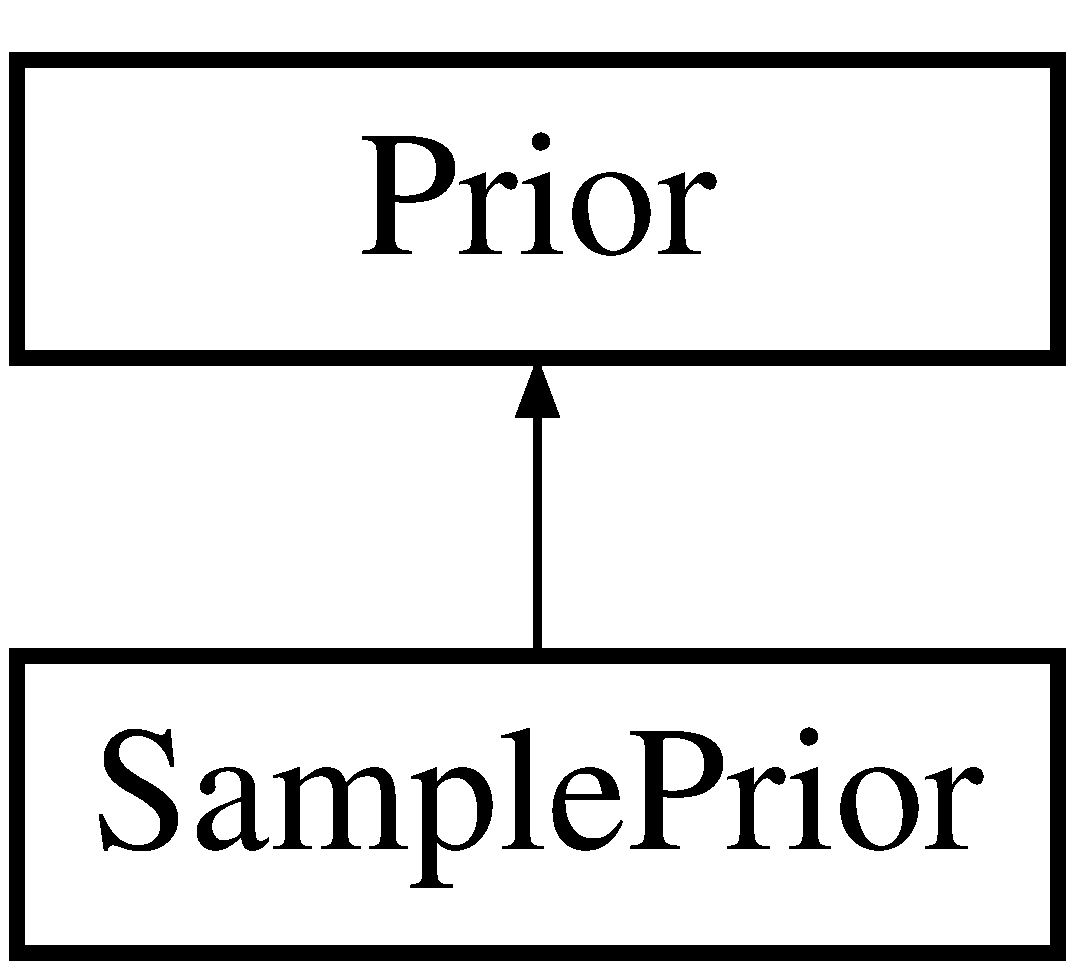
\includegraphics[height=2.000000cm]{classPrior}
\end{center}
\end{figure}
\subsection*{Public Member Functions}
\begin{DoxyCompactItemize}
\item 
virtual double \hyperlink{classPrior_a4c130ca9913663eb13d423045640345f}{evaluate} (P\-Chain $\ast$protein)
\begin{DoxyCompactList}\small\item\em Override this function to define custom energy/prior function. \end{DoxyCompactList}\end{DoxyCompactItemize}


\subsection{Detailed Description}
Interface for user defined priors. 

\subsection{Member Function Documentation}
\hypertarget{classPrior_a4c130ca9913663eb13d423045640345f}{\index{Prior@{Prior}!evaluate@{evaluate}}
\index{evaluate@{evaluate}!Prior@{Prior}}
\subsubsection[{evaluate}]{\setlength{\rightskip}{0pt plus 5cm}double Prior\-::evaluate (
\begin{DoxyParamCaption}
\item[{P\-Chain $\ast$}]{protein}
\end{DoxyParamCaption}
)\hspace{0.3cm}{\ttfamily [virtual]}}}\label{classPrior_a4c130ca9913663eb13d423045640345f}


Override this function to define custom energy/prior function. 

\begin{DoxyReturn}{Returns}
Probability density in logarithm. 
\end{DoxyReturn}


Reimplemented in \hyperlink{classSamplePrior_af1209bf9710e4c336084c18b3eba3547}{Sample\-Prior}.



The documentation for this class was generated from the following files\-:\begin{DoxyCompactItemize}
\item 
Prior.\-h\item 
Prior.\-cc\end{DoxyCompactItemize}

\hypertarget{classProtein__Score}{\section{Protein\-\_\-\-Score Class Reference}
\label{classProtein__Score}\index{Protein\-\_\-\-Score@{Protein\-\_\-\-Score}}
}


An auxiliary class for class \hyperlink{classLoopTKSampler}{Loop\-T\-K\-Sampler}. This class is a data structure for storing a chain conformation and its score.  




{\ttfamily \#include $<$Loop\-T\-K\-Sampler.\-h$>$}

\subsection*{Public Attributes}
\begin{DoxyCompactItemize}
\item 
\hypertarget{classProtein__Score_a60756c2713d20bd5aaadd3f3e8005b7a}{P\-Protein $\ast$ {\bfseries protein}}\label{classProtein__Score_a60756c2713d20bd5aaadd3f3e8005b7a}

\item 
\hypertarget{classProtein__Score_a8e2b7edc38055d9e2efb9c93c8aae3c4}{double {\bfseries score}}\label{classProtein__Score_a8e2b7edc38055d9e2efb9c93c8aae3c4}

\end{DoxyCompactItemize}


\subsection{Detailed Description}
An auxiliary class for class \hyperlink{classLoopTKSampler}{Loop\-T\-K\-Sampler}. This class is a data structure for storing a chain conformation and its score. 

The documentation for this class was generated from the following file\-:\begin{DoxyCompactItemize}
\item 
Loop\-T\-K\-Sampler.\-h\end{DoxyCompactItemize}

\hypertarget{classRamachandranPlot}{\section{Ramachandran\-Plot Class Reference}
\label{classRamachandranPlot}\index{Ramachandran\-Plot@{Ramachandran\-Plot}}
}


The class \hyperlink{classRamachandranPlot}{Ramachandran\-Plot} is used to initialize and store database for Ramachandran plot, sample backbone dihedral angles according to residue type and evaluate the probability of one conformation according to backbone structure.  




{\ttfamily \#include $<$Ramachandran\-Plot.\-h$>$}

\subsection*{Public Member Functions}
\begin{DoxyCompactItemize}
\item 
\hyperlink{classRamachandranPlot_ab1c3ad4e59732c7b8800c7ebc616e125}{Ramachandran\-Plot} (int size=36, char $\ast$file\-\_\-pro=\char`\"{}../Data/\hyperlink{classRamachandranPlot}{Ramachandran\-Plot}/pro.\-txt\char`\"{}, char $\ast$file\-\_\-pre\-\_\-pro=\char`\"{}../Data/\hyperlink{classRamachandranPlot}{Ramachandran\-Plot}/pre\-\_\-pro.\-txt\char`\"{}, char $\ast$file\-\_\-gly=\char`\"{}../Data/\hyperlink{classRamachandranPlot}{Ramachandran\-Plot}/gly.\-txt\char`\"{}, char $\ast$file\-\_\-generic=\char`\"{}../Data/\hyperlink{classRamachandranPlot}{Ramachandran\-Plot}/gen.\-txt\char`\"{})
\begin{DoxyCompactList}\small\item\em Constructor. \end{DoxyCompactList}\item 
\hypertarget{classRamachandranPlot_a5f80329f5340a22a5c862dee94a81d42}{virtual \hyperlink{classRamachandranPlot_a5f80329f5340a22a5c862dee94a81d42}{$\sim$\-Ramachandran\-Plot} ()}\label{classRamachandranPlot_a5f80329f5340a22a5c862dee94a81d42}

\begin{DoxyCompactList}\small\item\em Destructor. \end{DoxyCompactList}\item 
Dihedral\-Angle $\ast$ \hyperlink{classRamachandranPlot_a73249700e3ac5ff556de348eb46224bc}{get\-Random\-Dihedral\-Angle} (int type)
\begin{DoxyCompactList}\small\item\em Randomly generate a pair of backbone dihedral angles of specific type. \end{DoxyCompactList}\item 
Dihedral\-Angle $\ast$ \hyperlink{classRamachandranPlot_a389830f21dbca4084c854f797718a922}{get\-Random\-Dihedral\-Angle} (string name, string name\-\_\-next)
\begin{DoxyCompactList}\small\item\em Randomly generate a pair of backbone dihedral angles given residue name. \end{DoxyCompactList}\item 
double \hyperlink{classRamachandranPlot_a37be1f0f5adbbf0bc00ba678a910d365}{get\-Residue\-Angle\-Probability} (P\-Chain $\ast$chain, int index)
\begin{DoxyCompactList}\small\item\em Evaluate the probability of a residue's structure according to Ramachandran plot. \end{DoxyCompactList}\end{DoxyCompactItemize}
\subsection*{Static Public Attributes}
\begin{DoxyCompactItemize}
\item 
\hypertarget{classRamachandranPlot_a2dbb64dc6f788952b725d8401c0936e0}{static const int {\bfseries P\-R\-O} = 0}\label{classRamachandranPlot_a2dbb64dc6f788952b725d8401c0936e0}

\item 
\hypertarget{classRamachandranPlot_a975ab2d49eeb7cf60a7b6b990cb2c706}{static const int {\bfseries P\-R\-E\-\_\-\-P\-R\-O} = 1}\label{classRamachandranPlot_a975ab2d49eeb7cf60a7b6b990cb2c706}

\item 
\hypertarget{classRamachandranPlot_a26a068e7bfe44b31d4f74128260f500f}{static const int {\bfseries G\-L\-Y} = 2}\label{classRamachandranPlot_a26a068e7bfe44b31d4f74128260f500f}

\item 
\hypertarget{classRamachandranPlot_af0c0a68977085e86138c6adf32ed9753}{static const int {\bfseries G\-E\-N\-E\-R\-I\-C} = 3}\label{classRamachandranPlot_af0c0a68977085e86138c6adf32ed9753}

\end{DoxyCompactItemize}
\subsection*{Private Member Functions}
\begin{DoxyCompactItemize}
\item 
double $\ast$ \hyperlink{classRamachandranPlot_a742cd67cdd45fdeae7003958114b1502}{construct} (char $\ast$filename)
\begin{DoxyCompactList}\small\item\em Construct the Ramachandran plot. \end{DoxyCompactList}\end{DoxyCompactItemize}
\subsection*{Private Attributes}
\begin{DoxyCompactItemize}
\item 
\hypertarget{classRamachandranPlot_a975823bb2e3b12fd5e58207075b04e26}{double $\ast$ {\bfseries pro\-\_\-acc}}\label{classRamachandranPlot_a975823bb2e3b12fd5e58207075b04e26}

\item 
\hypertarget{classRamachandranPlot_aa6410400501b566f1d6f6076367f528e}{double $\ast$ {\bfseries pre\-\_\-pro\-\_\-acc}}\label{classRamachandranPlot_aa6410400501b566f1d6f6076367f528e}

\item 
\hypertarget{classRamachandranPlot_a998af9bca9f9e0e867686b011a68f3c6}{double $\ast$ {\bfseries gly\-\_\-acc}}\label{classRamachandranPlot_a998af9bca9f9e0e867686b011a68f3c6}

\item 
\hypertarget{classRamachandranPlot_aebc3a87f98922bae0036216d554225f8}{double $\ast$ {\bfseries gen\-\_\-acc}}\label{classRamachandranPlot_aebc3a87f98922bae0036216d554225f8}

\item 
\hypertarget{classRamachandranPlot_af46818df510f286feaf84c2ff3d64727}{double $\ast$ {\bfseries pro}}\label{classRamachandranPlot_af46818df510f286feaf84c2ff3d64727}

\item 
\hypertarget{classRamachandranPlot_a916665cc07de5f6c84d8b9b42bc20ec5}{double $\ast$ {\bfseries pre\-\_\-pro}}\label{classRamachandranPlot_a916665cc07de5f6c84d8b9b42bc20ec5}

\item 
\hypertarget{classRamachandranPlot_abf0f243922afede50c65af2d5360bc91}{double $\ast$ {\bfseries gly}}\label{classRamachandranPlot_abf0f243922afede50c65af2d5360bc91}

\item 
\hypertarget{classRamachandranPlot_ad4461154c24da389d49b3f13856babdc}{double $\ast$ {\bfseries gen}}\label{classRamachandranPlot_ad4461154c24da389d49b3f13856babdc}

\item 
\hypertarget{classRamachandranPlot_abb1b9899449d15f084fee1b1c51ca418}{int {\bfseries size}}\label{classRamachandranPlot_abb1b9899449d15f084fee1b1c51ca418}

\item 
\hypertarget{classRamachandranPlot_a1ef03baf68e4595fd7bdd6db269b3ffa}{int {\bfseries gridnum}}\label{classRamachandranPlot_a1ef03baf68e4595fd7bdd6db269b3ffa}

\item 
\hypertarget{classRamachandranPlot_a608705177e4171c0488071468b3df216}{double {\bfseries gridlength}}\label{classRamachandranPlot_a608705177e4171c0488071468b3df216}

\end{DoxyCompactItemize}


\subsection{Detailed Description}
The class \hyperlink{classRamachandranPlot}{Ramachandran\-Plot} is used to initialize and store database for Ramachandran plot, sample backbone dihedral angles according to residue type and evaluate the probability of one conformation according to backbone structure. 

\subsection{Constructor \& Destructor Documentation}
\hypertarget{classRamachandranPlot_ab1c3ad4e59732c7b8800c7ebc616e125}{\index{Ramachandran\-Plot@{Ramachandran\-Plot}!Ramachandran\-Plot@{Ramachandran\-Plot}}
\index{Ramachandran\-Plot@{Ramachandran\-Plot}!RamachandranPlot@{Ramachandran\-Plot}}
\subsubsection[{Ramachandran\-Plot}]{\setlength{\rightskip}{0pt plus 5cm}Ramachandran\-Plot\-::\-Ramachandran\-Plot (
\begin{DoxyParamCaption}
\item[{int}]{size = {\ttfamily 36}, }
\item[{char $\ast$}]{file\-\_\-pro = {\ttfamily \char`\"{}../Data/{\bf Ramachandran\-Plot}/pro.txt\char`\"{}}, }
\item[{char $\ast$}]{file\-\_\-pre\-\_\-pro = {\ttfamily \char`\"{}../Data/{\bf Ramachandran\-Plot}/pre\-\_\-pro.txt\char`\"{}}, }
\item[{char $\ast$}]{file\-\_\-gly = {\ttfamily \char`\"{}../Data/{\bf Ramachandran\-Plot}/gly.txt\char`\"{}}, }
\item[{char $\ast$}]{file\-\_\-generic = {\ttfamily \char`\"{}../Data/{\bf Ramachandran\-Plot}/gen.txt\char`\"{}}}
\end{DoxyParamCaption}
)}}\label{classRamachandranPlot_ab1c3ad4e59732c7b8800c7ebc616e125}


Constructor. 


\begin{DoxyParams}{Parameters}
{\em size} & number of grids to discretize the angle space \mbox{[}-\/180.\-0, 180.\-0\mbox{]}. By default, 10-\/degree is the width of a grid. \\
\hline
{\em file\-\_\-pro} & library location for Proline \\
\hline
{\em file\-\_\-pre\-\_\-pro} & library location for pre-\/\-Prolines \\
\hline
{\em file\-\_\-gly} & library location for Glycine \\
\hline
{\em file\-\_\-generic} & library location for generic residues \\
\hline
\end{DoxyParams}


\subsection{Member Function Documentation}
\hypertarget{classRamachandranPlot_a742cd67cdd45fdeae7003958114b1502}{\index{Ramachandran\-Plot@{Ramachandran\-Plot}!construct@{construct}}
\index{construct@{construct}!RamachandranPlot@{Ramachandran\-Plot}}
\subsubsection[{construct}]{\setlength{\rightskip}{0pt plus 5cm}double $\ast$ Ramachandran\-Plot\-::construct (
\begin{DoxyParamCaption}
\item[{char $\ast$}]{filename}
\end{DoxyParamCaption}
)\hspace{0.3cm}{\ttfamily [private]}}}\label{classRamachandranPlot_a742cd67cdd45fdeae7003958114b1502}


Construct the Ramachandran plot. 


\begin{DoxyParams}{Parameters}
{\em filename} & data file \\
\hline
\end{DoxyParams}
\begin{DoxyReturn}{Returns}
a database 
\end{DoxyReturn}
\hypertarget{classRamachandranPlot_a73249700e3ac5ff556de348eb46224bc}{\index{Ramachandran\-Plot@{Ramachandran\-Plot}!get\-Random\-Dihedral\-Angle@{get\-Random\-Dihedral\-Angle}}
\index{get\-Random\-Dihedral\-Angle@{get\-Random\-Dihedral\-Angle}!RamachandranPlot@{Ramachandran\-Plot}}
\subsubsection[{get\-Random\-Dihedral\-Angle}]{\setlength{\rightskip}{0pt plus 5cm}Dihedral\-Angle $\ast$ Ramachandran\-Plot\-::get\-Random\-Dihedral\-Angle (
\begin{DoxyParamCaption}
\item[{int}]{type}
\end{DoxyParamCaption}
)}}\label{classRamachandranPlot_a73249700e3ac5ff556de348eb46224bc}


Randomly generate a pair of backbone dihedral angles of specific type. 


\begin{DoxyParams}{Parameters}
{\em type} & residue type \{P\-R\-O, P\-R\-E\-\_\-\-P\-R\-O, G\-L\-Y, G\-E\-N\-E\-R\-I\-C\} \\
\hline
\end{DoxyParams}
\begin{DoxyReturn}{Returns}
a pair of dihedral angles 
\end{DoxyReturn}
\hypertarget{classRamachandranPlot_a389830f21dbca4084c854f797718a922}{\index{Ramachandran\-Plot@{Ramachandran\-Plot}!get\-Random\-Dihedral\-Angle@{get\-Random\-Dihedral\-Angle}}
\index{get\-Random\-Dihedral\-Angle@{get\-Random\-Dihedral\-Angle}!RamachandranPlot@{Ramachandran\-Plot}}
\subsubsection[{get\-Random\-Dihedral\-Angle}]{\setlength{\rightskip}{0pt plus 5cm}Dihedral\-Angle $\ast$ Ramachandran\-Plot\-::get\-Random\-Dihedral\-Angle (
\begin{DoxyParamCaption}
\item[{string}]{name, }
\item[{string}]{name\-\_\-next}
\end{DoxyParamCaption}
)}}\label{classRamachandranPlot_a389830f21dbca4084c854f797718a922}


Randomly generate a pair of backbone dihedral angles given residue name. 


\begin{DoxyParams}{Parameters}
{\em name} & name of the residue \\
\hline
{\em name\-\_\-next} & name of the succeeding residue (for pre-\/\-Pro residues) \\
\hline
\end{DoxyParams}
\begin{DoxyReturn}{Returns}
a pair of dihedral angles 
\end{DoxyReturn}
\hypertarget{classRamachandranPlot_a37be1f0f5adbbf0bc00ba678a910d365}{\index{Ramachandran\-Plot@{Ramachandran\-Plot}!get\-Residue\-Angle\-Probability@{get\-Residue\-Angle\-Probability}}
\index{get\-Residue\-Angle\-Probability@{get\-Residue\-Angle\-Probability}!RamachandranPlot@{Ramachandran\-Plot}}
\subsubsection[{get\-Residue\-Angle\-Probability}]{\setlength{\rightskip}{0pt plus 5cm}double Ramachandran\-Plot\-::get\-Residue\-Angle\-Probability (
\begin{DoxyParamCaption}
\item[{P\-Chain $\ast$}]{chain, }
\item[{int}]{index}
\end{DoxyParamCaption}
)}}\label{classRamachandranPlot_a37be1f0f5adbbf0bc00ba678a910d365}


Evaluate the probability of a residue's structure according to Ramachandran plot. 


\begin{DoxyParams}{Parameters}
{\em chain} & the chain which contains the residue \\
\hline
{\em index} & the index of the residue in the chain \\
\hline
\end{DoxyParams}
\begin{DoxyReturn}{Returns}
probability of the residue structure 
\end{DoxyReturn}


The documentation for this class was generated from the following files\-:\begin{DoxyCompactItemize}
\item 
Ramachandran\-Plot.\-h\item 
Ramachandran\-Plot.\-cc\end{DoxyCompactItemize}

\hypertarget{classRandom}{\section{Random Class Reference}
\label{classRandom}\index{Random@{Random}}
}


An auxiliary class. The class is used for generating random values.  




{\ttfamily \#include $<$Utility.\-h$>$}

\subsection*{Static Public Member Functions}
\begin{DoxyCompactItemize}
\item 
static int \hyperlink{classRandom_a087f0acc28943cb0d2972f649a7157e4}{next\-Int} (const int r)
\begin{DoxyCompactList}\small\item\em Get a random integer from 0 to r -\/ 1. \end{DoxyCompactList}\item 
static int \hyperlink{classRandom_a5c90ef3456529a033571d01435e84f4d}{next\-Int} (const int r1, const int r2)
\begin{DoxyCompactList}\small\item\em Get a random integer from r1 to r2. \end{DoxyCompactList}\item 
static double \hyperlink{classRandom_a92ff638325ddfa7bafb1a17dd61db5ee}{next\-Double} (const double range)
\begin{DoxyCompactList}\small\item\em Get a random double from 0 to range. \end{DoxyCompactList}\item 
static double \hyperlink{classRandom_aeb0767ec85429c66f25035ddb4cce885}{next\-Double} (const double r1, const double r2)
\begin{DoxyCompactList}\small\item\em Get a random double from r1 to r2. \end{DoxyCompactList}\item 
static double \hyperlink{classRandom_aa0890fcdcc1173fffc223d7a2bf84324}{next\-Normal} ()
\begin{DoxyCompactList}\small\item\em Draw a random value from normal distribution N( 0, 1) \end{DoxyCompactList}\item 
static double \hyperlink{classRandom_a21be54b4bb78f9006292dd290a6e69bf}{next\-Normal} (const double mean, const double std)
\begin{DoxyCompactList}\small\item\em Draw a random value from normal distribution N( mean, std $\ast$ std) \end{DoxyCompactList}\end{DoxyCompactItemize}


\subsection{Detailed Description}
An auxiliary class. The class is used for generating random values. 

\subsection{Member Function Documentation}
\hypertarget{classRandom_a92ff638325ddfa7bafb1a17dd61db5ee}{\index{Random@{Random}!next\-Double@{next\-Double}}
\index{next\-Double@{next\-Double}!Random@{Random}}
\subsubsection[{next\-Double}]{\setlength{\rightskip}{0pt plus 5cm}double Random\-::next\-Double (
\begin{DoxyParamCaption}
\item[{const double}]{range}
\end{DoxyParamCaption}
)\hspace{0.3cm}{\ttfamily [static]}}}\label{classRandom_a92ff638325ddfa7bafb1a17dd61db5ee}


Get a random double from 0 to range. 


\begin{DoxyParams}{Parameters}
{\em range} & upper bound \\
\hline
\end{DoxyParams}
\begin{DoxyReturn}{Returns}
a double value 
\end{DoxyReturn}
\hypertarget{classRandom_aeb0767ec85429c66f25035ddb4cce885}{\index{Random@{Random}!next\-Double@{next\-Double}}
\index{next\-Double@{next\-Double}!Random@{Random}}
\subsubsection[{next\-Double}]{\setlength{\rightskip}{0pt plus 5cm}double Random\-::next\-Double (
\begin{DoxyParamCaption}
\item[{const double}]{r1, }
\item[{const double}]{r2}
\end{DoxyParamCaption}
)\hspace{0.3cm}{\ttfamily [static]}}}\label{classRandom_aeb0767ec85429c66f25035ddb4cce885}


Get a random double from r1 to r2. 


\begin{DoxyParams}{Parameters}
{\em r1} & lower bound \\
\hline
{\em r2} & upper bound \\
\hline
\end{DoxyParams}
\begin{DoxyReturn}{Returns}
a double value 
\end{DoxyReturn}
\hypertarget{classRandom_a087f0acc28943cb0d2972f649a7157e4}{\index{Random@{Random}!next\-Int@{next\-Int}}
\index{next\-Int@{next\-Int}!Random@{Random}}
\subsubsection[{next\-Int}]{\setlength{\rightskip}{0pt plus 5cm}int Random\-::next\-Int (
\begin{DoxyParamCaption}
\item[{const int}]{r}
\end{DoxyParamCaption}
)\hspace{0.3cm}{\ttfamily [static]}}}\label{classRandom_a087f0acc28943cb0d2972f649a7157e4}


Get a random integer from 0 to r -\/ 1. 


\begin{DoxyParams}{Parameters}
{\em r} & upper bound of integer value (exclusive) \\
\hline
\end{DoxyParams}
\begin{DoxyReturn}{Returns}
an integer 
\end{DoxyReturn}
\hypertarget{classRandom_a5c90ef3456529a033571d01435e84f4d}{\index{Random@{Random}!next\-Int@{next\-Int}}
\index{next\-Int@{next\-Int}!Random@{Random}}
\subsubsection[{next\-Int}]{\setlength{\rightskip}{0pt plus 5cm}int Random\-::next\-Int (
\begin{DoxyParamCaption}
\item[{const int}]{r1, }
\item[{const int}]{r2}
\end{DoxyParamCaption}
)\hspace{0.3cm}{\ttfamily [static]}}}\label{classRandom_a5c90ef3456529a033571d01435e84f4d}


Get a random integer from r1 to r2. 


\begin{DoxyParams}{Parameters}
{\em r1} & tight lower bound \\
\hline
{\em r2} & tight upper bound \\
\hline
\end{DoxyParams}
\begin{DoxyReturn}{Returns}
an integer 
\end{DoxyReturn}
\hypertarget{classRandom_aa0890fcdcc1173fffc223d7a2bf84324}{\index{Random@{Random}!next\-Normal@{next\-Normal}}
\index{next\-Normal@{next\-Normal}!Random@{Random}}
\subsubsection[{next\-Normal}]{\setlength{\rightskip}{0pt plus 5cm}double Random\-::next\-Normal (
\begin{DoxyParamCaption}
{}
\end{DoxyParamCaption}
)\hspace{0.3cm}{\ttfamily [static]}}}\label{classRandom_aa0890fcdcc1173fffc223d7a2bf84324}


Draw a random value from normal distribution N( 0, 1) 

\begin{DoxyReturn}{Returns}
a double value 
\end{DoxyReturn}
\hypertarget{classRandom_a21be54b4bb78f9006292dd290a6e69bf}{\index{Random@{Random}!next\-Normal@{next\-Normal}}
\index{next\-Normal@{next\-Normal}!Random@{Random}}
\subsubsection[{next\-Normal}]{\setlength{\rightskip}{0pt plus 5cm}double Random\-::next\-Normal (
\begin{DoxyParamCaption}
\item[{const double}]{mean, }
\item[{const double}]{std}
\end{DoxyParamCaption}
)\hspace{0.3cm}{\ttfamily [static]}}}\label{classRandom_a21be54b4bb78f9006292dd290a6e69bf}


Draw a random value from normal distribution N( mean, std $\ast$ std) 


\begin{DoxyParams}{Parameters}
{\em mean} & mean of normal distribution \\
\hline
{\em std} & standard deviation of normal distribution \\
\hline
\end{DoxyParams}
\begin{DoxyReturn}{Returns}
a double value 
\end{DoxyReturn}


The documentation for this class was generated from the following files\-:\begin{DoxyCompactItemize}
\item 
Utility.\-h\item 
Utility.\-cc\end{DoxyCompactItemize}

\hypertarget{classRotamer}{\section{Rotamer Class Reference}
\label{classRotamer}\index{Rotamer@{Rotamer}}
}


The class \hyperlink{classRotamer}{Rotamer} is used to initialize side-\/chain database by parsing Dunbrack's Backbone Dependent \hyperlink{classRotamer}{Rotamer} Library, sample one side-\/chain conformation for a given residue, evaluate the probability given one side-\/chain conformation.  




{\ttfamily \#include $<$Rotamer.\-h$>$}

\subsection*{Public Member Functions}
\begin{DoxyCompactItemize}
\item 
\hyperlink{classRotamer_a9646e84497feedfb6a09ff9937cb4313}{Rotamer} (P\-Protein $\ast$protein)
\item 
void \hyperlink{classRotamer_a2938ad7d918e69f6f71f3a42a3019b35}{sample} (const string \&residue\-\_\-name, const double \&phi, const double \&psi, int \&rotamer\-\_\-grid, vector$<$ double $>$ \&d\-Angles)
\begin{DoxyCompactList}\small\item\em Randomly sample side-\/chain chi angles given residue name and backbone dihedral angle pair. \end{DoxyCompactList}\item 
void \hyperlink{classRotamer_aa58ff58cc11cfe9a68376e5b99ae3b51}{sample\-\_\-common} (const string \&residue\-\_\-name, const int \&phi, const int \&psi, int \&rotamer\-\_\-grid, vector$<$ double $>$ \&d\-Angles)
\begin{DoxyCompactList}\small\item\em Randomly sample side-\/chain chi angles given rotameric residue name and backbone dihedral angle pair. \end{DoxyCompactList}\item 
void \hyperlink{classRotamer_a062044d5ca99c307fb6be2369ed200bf}{sample\-\_\-\-Special} (const string \&residue\-\_\-name, const int \&phi, const int \&psi, int \&rotamer\-\_\-grid, vector$<$ double $>$ \&d\-Angles)
\begin{DoxyCompactList}\small\item\em Randomly sample side-\/chain chi angles given non-\/rotameric residue name and backbone dihedral angle pair. \end{DoxyCompactList}\item 
void \hyperlink{classRotamer_a9714326d4ad191c22e4672a6e5e8355d}{output} (char $\ast$filename)
\begin{DoxyCompactList}\small\item\em Output the database to a file. \end{DoxyCompactList}\item 
double \hyperlink{classRotamer_a813f284c56b83a9fe8d33ac82707954a}{eval\-Sidechain\-\_\-log} (P\-Chain $\ast$chain, const int s, const int e)
\begin{DoxyCompactList}\small\item\em Evaluate side-\/chain structures given one protein chain. \end{DoxyCompactList}\item 
void \hyperlink{classRotamer_a0b585070951b6afb654f41703a5bf695}{init\-Sidechain\-Database} (P\-Protein $\ast$protein)
\begin{DoxyCompactList}\small\item\em Initialize sidechain database according to residues the protein contains. \end{DoxyCompactList}\end{DoxyCompactItemize}
\subsection*{Private Member Functions}
\begin{DoxyCompactItemize}
\item 
\hypertarget{classRotamer_adefa784f73374d8733c3ad4f16b1d31c}{void {\bfseries init} ()}\label{classRotamer_adefa784f73374d8733c3ad4f16b1d31c}

\item 
void \hyperlink{classRotamer_a2d93b2979227b805045d511b1997d03c}{read} (const string \&res\-\_\-name)
\begin{DoxyCompactList}\small\item\em Read sidechain library given residue name and construct corresponding database. \end{DoxyCompactList}\item 
void \hyperlink{classRotamer_a7336f877be41970bef9323a037ad4b9b}{read\-\_\-common} (const string \&res\-\_\-name)
\begin{DoxyCompactList}\small\item\em Read sidechain library given the name of a rotameric residue and construct corresponding database. \end{DoxyCompactList}\item 
void \hyperlink{classRotamer_acc03226b45abfeac3f9c1ff15907871d}{read\-\_\-special} (const string \&res\-\_\-name)
\begin{DoxyCompactList}\small\item\em Read sidechain library given the name of a non-\/rotameric residue and construct corresponding database. \end{DoxyCompactList}\item 
int \hyperlink{classRotamer_a83414f9d04c442941780a44214358c64}{type} (const string \&res\-\_\-name)
\begin{DoxyCompactList}\small\item\em Return the type of residue given residue name. \end{DoxyCompactList}\item 
bool \hyperlink{classRotamer_a2210953e3efdc034621b1e346bccd353}{is\-Special} (const string \&res\-\_\-name)
\begin{DoxyCompactList}\small\item\em Check if the residue is rotameric or not. \end{DoxyCompactList}\end{DoxyCompactItemize}
\subsection*{Private Attributes}
\begin{DoxyCompactItemize}
\item 
\hypertarget{classRotamer_a76ee1c806449ead94fa3801e46e21e04}{Grid\-Map {\bfseries grid\-Map}}\label{classRotamer_a76ee1c806449ead94fa3801e46e21e04}

\item 
\hypertarget{classRotamer_aafeec4267c9e5574fff40c81510cc8d6}{Grid\-Map\-Special {\bfseries grid\-Map\-Special}}\label{classRotamer_aafeec4267c9e5574fff40c81510cc8d6}

\item 
\hypertarget{classRotamer_ac4070f518eddf3d53c778f0de4e588bf}{vector$<$ int $>$ {\bfseries degree\-\_\-start}}\label{classRotamer_ac4070f518eddf3d53c778f0de4e588bf}

\item 
\hypertarget{classRotamer_a4e9a547df84cb5b14d2428aedf14fbb1}{vector$<$ int $>$ {\bfseries degree\-\_\-end}}\label{classRotamer_a4e9a547df84cb5b14d2428aedf14fbb1}

\item 
\hypertarget{classRotamer_af4c4d542df7ea52375a4dc1fd25f4425}{vector$<$ int $>$ {\bfseries step\-Length}}\label{classRotamer_af4c4d542df7ea52375a4dc1fd25f4425}

\item 
\hypertarget{classRotamer_a2a3f5f9eb1cb68fbe5a76c8b409b386d}{map$<$ string, int $>$ {\bfseries type\-Map}}\label{classRotamer_a2a3f5f9eb1cb68fbe5a76c8b409b386d}

\end{DoxyCompactItemize}
\subsection*{Static Private Attributes}
\begin{DoxyCompactItemize}
\item 
\hypertarget{classRotamer_a74531505f22df04f9cc8f6f1a9446b43}{static const int {\bfseries A\-S\-N} = 0}\label{classRotamer_a74531505f22df04f9cc8f6f1a9446b43}

\item 
\hypertarget{classRotamer_ab4e8dc3cd5bb7af8b9034b60551107cd}{static const int {\bfseries A\-S\-P} = 1}\label{classRotamer_ab4e8dc3cd5bb7af8b9034b60551107cd}

\item 
\hypertarget{classRotamer_aa4134daf455c87b5125a09a92557150b}{static const int {\bfseries P\-H\-E} = 2}\label{classRotamer_aa4134daf455c87b5125a09a92557150b}

\item 
\hypertarget{classRotamer_a81006b4b69528bde0da59807cd8337d8}{static const int {\bfseries T\-R\-P} = 3}\label{classRotamer_a81006b4b69528bde0da59807cd8337d8}

\item 
\hypertarget{classRotamer_a8182f9506799c4804996fcaab1998e3e}{static const int {\bfseries H\-I\-S} = 4}\label{classRotamer_a8182f9506799c4804996fcaab1998e3e}

\item 
\hypertarget{classRotamer_a34e69bdbf3bb7e75514cbca1382dd783}{static const int {\bfseries T\-Y\-R} = 5}\label{classRotamer_a34e69bdbf3bb7e75514cbca1382dd783}

\item 
\hypertarget{classRotamer_ab6344892c9b56fae3485b98c88f569f3}{static const int {\bfseries G\-L\-N} = 6}\label{classRotamer_ab6344892c9b56fae3485b98c88f569f3}

\item 
\hypertarget{classRotamer_aec53b6e0a7f4e5bba337eb8ba3239132}{static const int {\bfseries G\-L\-U} = 7}\label{classRotamer_aec53b6e0a7f4e5bba337eb8ba3239132}

\end{DoxyCompactItemize}


\subsection{Detailed Description}
The class \hyperlink{classRotamer}{Rotamer} is used to initialize side-\/chain database by parsing Dunbrack's Backbone Dependent \hyperlink{classRotamer}{Rotamer} Library, sample one side-\/chain conformation for a given residue, evaluate the probability given one side-\/chain conformation. 

\subsection{Constructor \& Destructor Documentation}
\hypertarget{classRotamer_a9646e84497feedfb6a09ff9937cb4313}{\index{Rotamer@{Rotamer}!Rotamer@{Rotamer}}
\index{Rotamer@{Rotamer}!Rotamer@{Rotamer}}
\subsubsection[{Rotamer}]{\setlength{\rightskip}{0pt plus 5cm}Rotamer\-::\-Rotamer (
\begin{DoxyParamCaption}
\item[{P\-Protein $\ast$}]{protein}
\end{DoxyParamCaption}
)}}\label{classRotamer_a9646e84497feedfb6a09ff9937cb4313}

\begin{DoxyParams}{Parameters}
{\em protein} & protein chain to be sampled \\
\hline
\end{DoxyParams}


\subsection{Member Function Documentation}
\hypertarget{classRotamer_a813f284c56b83a9fe8d33ac82707954a}{\index{Rotamer@{Rotamer}!eval\-Sidechain\-\_\-log@{eval\-Sidechain\-\_\-log}}
\index{eval\-Sidechain\-\_\-log@{eval\-Sidechain\-\_\-log}!Rotamer@{Rotamer}}
\subsubsection[{eval\-Sidechain\-\_\-log}]{\setlength{\rightskip}{0pt plus 5cm}double Rotamer\-::eval\-Sidechain\-\_\-log (
\begin{DoxyParamCaption}
\item[{P\-Chain $\ast$}]{chain, }
\item[{const int}]{s, }
\item[{const int}]{e}
\end{DoxyParamCaption}
)}}\label{classRotamer_a813f284c56b83a9fe8d33ac82707954a}


Evaluate side-\/chain structures given one protein chain. 


\begin{DoxyParams}{Parameters}
{\em chain} & protein chain to be evaluated \\
\hline
{\em s} & index of starting residue in protein chain \\
\hline
{\em e} & index of ending residue in protein chain \\
\hline
\end{DoxyParams}
\begin{DoxyReturn}{Returns}
probability density in logarithm 
\end{DoxyReturn}
\hypertarget{classRotamer_a0b585070951b6afb654f41703a5bf695}{\index{Rotamer@{Rotamer}!init\-Sidechain\-Database@{init\-Sidechain\-Database}}
\index{init\-Sidechain\-Database@{init\-Sidechain\-Database}!Rotamer@{Rotamer}}
\subsubsection[{init\-Sidechain\-Database}]{\setlength{\rightskip}{0pt plus 5cm}void Rotamer\-::init\-Sidechain\-Database (
\begin{DoxyParamCaption}
\item[{P\-Protein $\ast$}]{protein}
\end{DoxyParamCaption}
)}}\label{classRotamer_a0b585070951b6afb654f41703a5bf695}


Initialize sidechain database according to residues the protein contains. 


\begin{DoxyParams}{Parameters}
{\em protein} & protein chain to be sampled \\
\hline
\end{DoxyParams}
\hypertarget{classRotamer_a2210953e3efdc034621b1e346bccd353}{\index{Rotamer@{Rotamer}!is\-Special@{is\-Special}}
\index{is\-Special@{is\-Special}!Rotamer@{Rotamer}}
\subsubsection[{is\-Special}]{\setlength{\rightskip}{0pt plus 5cm}bool Rotamer\-::is\-Special (
\begin{DoxyParamCaption}
\item[{const string \&}]{res\-\_\-name}
\end{DoxyParamCaption}
)\hspace{0.3cm}{\ttfamily [private]}}}\label{classRotamer_a2210953e3efdc034621b1e346bccd353}


Check if the residue is rotameric or not. 


\begin{DoxyParams}{Parameters}
{\em res\-\_\-name} & residue name \\
\hline
\end{DoxyParams}
\begin{DoxyReturn}{Returns}
true, rotemeric; false, non-\/rotameric 
\end{DoxyReturn}
\hypertarget{classRotamer_a9714326d4ad191c22e4672a6e5e8355d}{\index{Rotamer@{Rotamer}!output@{output}}
\index{output@{output}!Rotamer@{Rotamer}}
\subsubsection[{output}]{\setlength{\rightskip}{0pt plus 5cm}void Rotamer\-::output (
\begin{DoxyParamCaption}
\item[{char $\ast$}]{filename}
\end{DoxyParamCaption}
)}}\label{classRotamer_a9714326d4ad191c22e4672a6e5e8355d}


Output the database to a file. 


\begin{DoxyParams}{Parameters}
{\em filename} & output filename \\
\hline
\end{DoxyParams}
\hypertarget{classRotamer_a2d93b2979227b805045d511b1997d03c}{\index{Rotamer@{Rotamer}!read@{read}}
\index{read@{read}!Rotamer@{Rotamer}}
\subsubsection[{read}]{\setlength{\rightskip}{0pt plus 5cm}void Rotamer\-::read (
\begin{DoxyParamCaption}
\item[{const string \&}]{res\-\_\-name}
\end{DoxyParamCaption}
)\hspace{0.3cm}{\ttfamily [private]}}}\label{classRotamer_a2d93b2979227b805045d511b1997d03c}


Read sidechain library given residue name and construct corresponding database. 


\begin{DoxyParams}{Parameters}
{\em res\-\_\-name} & residue name \\
\hline
\end{DoxyParams}
\hypertarget{classRotamer_a7336f877be41970bef9323a037ad4b9b}{\index{Rotamer@{Rotamer}!read\-\_\-common@{read\-\_\-common}}
\index{read\-\_\-common@{read\-\_\-common}!Rotamer@{Rotamer}}
\subsubsection[{read\-\_\-common}]{\setlength{\rightskip}{0pt plus 5cm}void Rotamer\-::read\-\_\-common (
\begin{DoxyParamCaption}
\item[{const string \&}]{res\-\_\-name}
\end{DoxyParamCaption}
)\hspace{0.3cm}{\ttfamily [private]}}}\label{classRotamer_a7336f877be41970bef9323a037ad4b9b}


Read sidechain library given the name of a rotameric residue and construct corresponding database. 


\begin{DoxyParams}{Parameters}
{\em res\-\_\-name} & residue name \\
\hline
\end{DoxyParams}
\hypertarget{classRotamer_acc03226b45abfeac3f9c1ff15907871d}{\index{Rotamer@{Rotamer}!read\-\_\-special@{read\-\_\-special}}
\index{read\-\_\-special@{read\-\_\-special}!Rotamer@{Rotamer}}
\subsubsection[{read\-\_\-special}]{\setlength{\rightskip}{0pt plus 5cm}void Rotamer\-::read\-\_\-special (
\begin{DoxyParamCaption}
\item[{const string \&}]{res\-\_\-name}
\end{DoxyParamCaption}
)\hspace{0.3cm}{\ttfamily [private]}}}\label{classRotamer_acc03226b45abfeac3f9c1ff15907871d}


Read sidechain library given the name of a non-\/rotameric residue and construct corresponding database. 


\begin{DoxyParams}{Parameters}
{\em res\-\_\-name} & residue name \\
\hline
\end{DoxyParams}
\hypertarget{classRotamer_a2938ad7d918e69f6f71f3a42a3019b35}{\index{Rotamer@{Rotamer}!sample@{sample}}
\index{sample@{sample}!Rotamer@{Rotamer}}
\subsubsection[{sample}]{\setlength{\rightskip}{0pt plus 5cm}void Rotamer\-::sample (
\begin{DoxyParamCaption}
\item[{const string \&}]{residue\-\_\-name, }
\item[{const double \&}]{phi, }
\item[{const double \&}]{psi, }
\item[{int \&}]{rotamer\-\_\-grid, }
\item[{vector$<$ double $>$ \&}]{d\-Angles}
\end{DoxyParamCaption}
)}}\label{classRotamer_a2938ad7d918e69f6f71f3a42a3019b35}


Randomly sample side-\/chain chi angles given residue name and backbone dihedral angle pair. 


\begin{DoxyParams}{Parameters}
{\em residue\-\_\-name} & name of the residue \\
\hline
{\em phi} & backbone phi angle \\
\hline
{\em psi} & backbone psi angle \\
\hline
{\em rotamer\-\_\-grid} & stores the grid index of rotamer in the rotamer database (for evaluation purpose) \\
\hline
{\em d\-Angles} & stores the side-\/chain chi angles \\
\hline
\end{DoxyParams}
\hypertarget{classRotamer_aa58ff58cc11cfe9a68376e5b99ae3b51}{\index{Rotamer@{Rotamer}!sample\-\_\-common@{sample\-\_\-common}}
\index{sample\-\_\-common@{sample\-\_\-common}!Rotamer@{Rotamer}}
\subsubsection[{sample\-\_\-common}]{\setlength{\rightskip}{0pt plus 5cm}void Rotamer\-::sample\-\_\-common (
\begin{DoxyParamCaption}
\item[{const string \&}]{residue\-\_\-name, }
\item[{const int \&}]{phi, }
\item[{const int \&}]{psi, }
\item[{int \&}]{rotamer\-\_\-grid, }
\item[{vector$<$ double $>$ \&}]{d\-Angles}
\end{DoxyParamCaption}
)}}\label{classRotamer_aa58ff58cc11cfe9a68376e5b99ae3b51}


Randomly sample side-\/chain chi angles given rotameric residue name and backbone dihedral angle pair. 


\begin{DoxyParams}{Parameters}
{\em residue\-\_\-name} & name of the residue \\
\hline
{\em phi} & backbone phi angle \\
\hline
{\em psi} & backbone psi angle \\
\hline
{\em rotamer\-\_\-grid} & stores the grid index of rotamer in the rotamer database (for evaluation purpose) \\
\hline
{\em d\-Angles} & stores the side-\/chain chi angles \\
\hline
\end{DoxyParams}
\hypertarget{classRotamer_a062044d5ca99c307fb6be2369ed200bf}{\index{Rotamer@{Rotamer}!sample\-\_\-\-Special@{sample\-\_\-\-Special}}
\index{sample\-\_\-\-Special@{sample\-\_\-\-Special}!Rotamer@{Rotamer}}
\subsubsection[{sample\-\_\-\-Special}]{\setlength{\rightskip}{0pt plus 5cm}void Rotamer\-::sample\-\_\-\-Special (
\begin{DoxyParamCaption}
\item[{const string \&}]{residue\-\_\-name, }
\item[{const int \&}]{phi, }
\item[{const int \&}]{psi, }
\item[{int \&}]{rotamer\-\_\-grid, }
\item[{vector$<$ double $>$ \&}]{d\-Angles}
\end{DoxyParamCaption}
)}}\label{classRotamer_a062044d5ca99c307fb6be2369ed200bf}


Randomly sample side-\/chain chi angles given non-\/rotameric residue name and backbone dihedral angle pair. 


\begin{DoxyParams}{Parameters}
{\em residue\-\_\-name} & name of the residue \\
\hline
{\em phi} & backbone phi angle \\
\hline
{\em psi} & backbone psi angle \\
\hline
{\em rotamer\-\_\-grid} & stores the grid index of rotamer in the rotamer database (for evaluation purpose) \\
\hline
{\em d\-Angles} & stores the side-\/chain chi angles \\
\hline
\end{DoxyParams}
\hypertarget{classRotamer_a83414f9d04c442941780a44214358c64}{\index{Rotamer@{Rotamer}!type@{type}}
\index{type@{type}!Rotamer@{Rotamer}}
\subsubsection[{type}]{\setlength{\rightskip}{0pt plus 5cm}int Rotamer\-::type (
\begin{DoxyParamCaption}
\item[{const string \&}]{res\-\_\-name}
\end{DoxyParamCaption}
)\hspace{0.3cm}{\ttfamily [private]}}}\label{classRotamer_a83414f9d04c442941780a44214358c64}


Return the type of residue given residue name. 

\begin{DoxyReturn}{Returns}
-\/1\-: rotameric residue; 0-\/7\-: A\-S\-N-\/\-G\-L\-U 
\end{DoxyReturn}


The documentation for this class was generated from the following files\-:\begin{DoxyCompactItemize}
\item 
Rotamer.\-h\item 
Rotamer.\-cc\end{DoxyCompactItemize}

\hypertarget{classRotamerGrid}{\section{Rotamer\-Grid Class Reference}
\label{classRotamerGrid}\index{Rotamer\-Grid@{Rotamer\-Grid}}
}


An auxilliary class for class \hyperlink{classRotamer}{Rotamer}. This class is a data structure for storing all rotamers in one dihedral angle grid.  




{\ttfamily \#include $<$Rotamer.\-h$>$}

Inheritance diagram for Rotamer\-Grid\-:\begin{figure}[H]
\begin{center}
\leavevmode
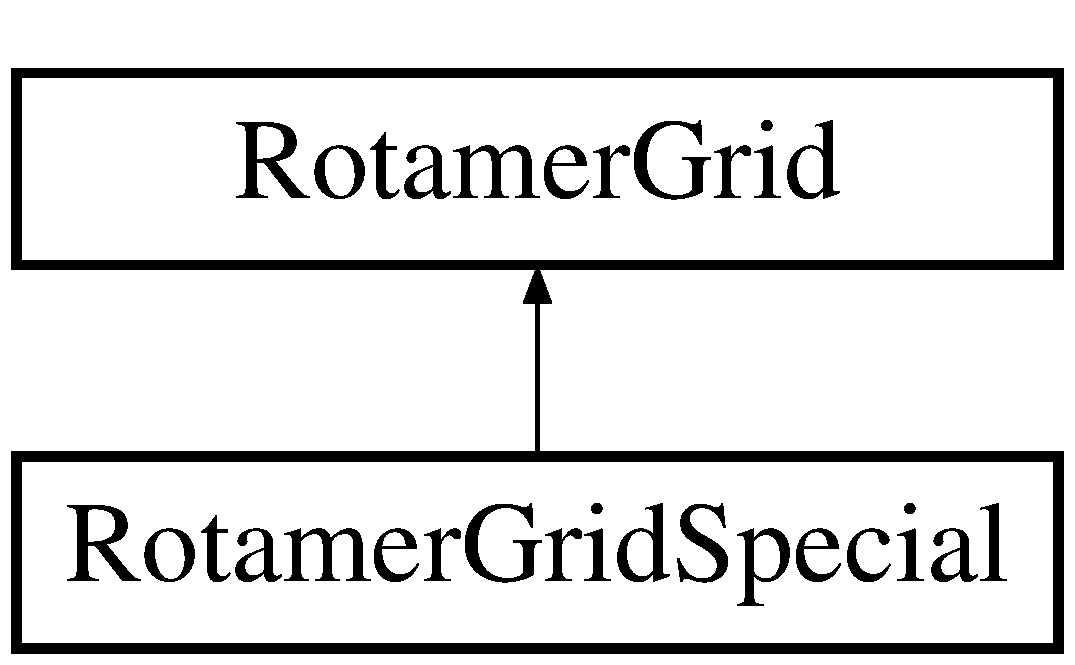
\includegraphics[height=2.000000cm]{classRotamerGrid}
\end{center}
\end{figure}
\subsection*{Public Attributes}
\begin{DoxyCompactItemize}
\item 
\hypertarget{classRotamerGrid_a93f842d1194d8b56c5b028a2acf391b3}{int {\bfseries n\-\_\-chi}}\label{classRotamerGrid_a93f842d1194d8b56c5b028a2acf391b3}

\item 
\hypertarget{classRotamerGrid_aaaf79beefd21e576d64eceb73bd78558}{vector$<$ double $>$ {\bfseries acc\-\_\-rotamer}}\label{classRotamerGrid_aaaf79beefd21e576d64eceb73bd78558}

\item 
\hypertarget{classRotamerGrid_aa82fe357e534c137dbd09216be3f24f7}{vector$<$ \hyperlink{classChiDistribution}{Chi\-Distribution} $>$ {\bfseries dist\-\_\-rotamer}}\label{classRotamerGrid_aa82fe357e534c137dbd09216be3f24f7}

\end{DoxyCompactItemize}
\subsection*{Friends}
\begin{DoxyCompactItemize}
\item 
\hypertarget{classRotamerGrid_abbb5e1f6ca569c67c8a354f8698eb62e}{class {\bfseries Rotamer}}\label{classRotamerGrid_abbb5e1f6ca569c67c8a354f8698eb62e}

\end{DoxyCompactItemize}


\subsection{Detailed Description}
An auxilliary class for class \hyperlink{classRotamer}{Rotamer}. This class is a data structure for storing all rotamers in one dihedral angle grid. 

The documentation for this class was generated from the following file\-:\begin{DoxyCompactItemize}
\item 
Rotamer.\-h\end{DoxyCompactItemize}

\hypertarget{classRotamerGridKey}{\section{Rotamer\-Grid\-Key Class Reference}
\label{classRotamerGridKey}\index{Rotamer\-Grid\-Key@{Rotamer\-Grid\-Key}}
}


An auxilliary class for class \hyperlink{classRotamer}{Rotamer}. This class used as a key to access one \hyperlink{classRotamerGrid}{Rotamer\-Grid} in the map structure.  




{\ttfamily \#include $<$Rotamer.\-h$>$}

\subsection*{Public Member Functions}
\begin{DoxyCompactItemize}
\item 
\hyperlink{classRotamerGridKey_aee87d6af570de7f03b485cbed293eb8d}{Rotamer\-Grid\-Key} (const string \&name, const int \&phi, const int \&psi)
\begin{DoxyCompactList}\small\item\em Constructor. \end{DoxyCompactList}\item 
string \hyperlink{classRotamerGridKey_ad88595feb7e0c7a4dbd0ac21936a4d11}{to\-String} () const 
\begin{DoxyCompactList}\small\item\em Get a string containing residue name, backbone phi and psi angles. \end{DoxyCompactList}\item 
\hypertarget{classRotamerGridKey_a3578afe99c7106457f0d89a71cb6ef17}{void \hyperlink{classRotamerGridKey_a3578afe99c7106457f0d89a71cb6ef17}{print} () const }\label{classRotamerGridKey_a3578afe99c7106457f0d89a71cb6ef17}

\begin{DoxyCompactList}\small\item\em Print the residue name, backbone phi,psi angles. \end{DoxyCompactList}\item 
bool \hyperlink{classRotamerGridKey_adf8cb8448cf8226bfa7272fcc4f2d1a6}{operator==} (const \hyperlink{classRotamerGridKey}{Rotamer\-Grid\-Key} \&key) const 
\begin{DoxyCompactList}\small\item\em \char`\"{}==\char`\"{} operator override to compare two Rotemer\-Grid\-Keys. \end{DoxyCompactList}\end{DoxyCompactItemize}
\subsection*{Private Attributes}
\begin{DoxyCompactItemize}
\item 
\hypertarget{classRotamerGridKey_a2d613cdc3ef66ac31971912f8a739820}{string {\bfseries name}}\label{classRotamerGridKey_a2d613cdc3ef66ac31971912f8a739820}

\item 
\hypertarget{classRotamerGridKey_a0077bcfd515e11fb1381858f96b58d70}{int {\bfseries phi}}\label{classRotamerGridKey_a0077bcfd515e11fb1381858f96b58d70}

\item 
\hypertarget{classRotamerGridKey_ab746864738cf575c10f8d0e2cd0fc20d}{int {\bfseries psi}}\label{classRotamerGridKey_ab746864738cf575c10f8d0e2cd0fc20d}

\end{DoxyCompactItemize}
\subsection*{Friends}
\begin{DoxyCompactItemize}
\item 
\hypertarget{classRotamerGridKey_abbb5e1f6ca569c67c8a354f8698eb62e}{class {\bfseries Rotamer}}\label{classRotamerGridKey_abbb5e1f6ca569c67c8a354f8698eb62e}

\item 
\hypertarget{classRotamerGridKey_a949353fe14fa04083e8cc7121c6f7d3e}{struct {\bfseries Rotamer\-Grid\-Key\-Comparator}}\label{classRotamerGridKey_a949353fe14fa04083e8cc7121c6f7d3e}

\end{DoxyCompactItemize}


\subsection{Detailed Description}
An auxilliary class for class \hyperlink{classRotamer}{Rotamer}. This class used as a key to access one \hyperlink{classRotamerGrid}{Rotamer\-Grid} in the map structure. 

\subsection{Constructor \& Destructor Documentation}
\hypertarget{classRotamerGridKey_aee87d6af570de7f03b485cbed293eb8d}{\index{Rotamer\-Grid\-Key@{Rotamer\-Grid\-Key}!Rotamer\-Grid\-Key@{Rotamer\-Grid\-Key}}
\index{Rotamer\-Grid\-Key@{Rotamer\-Grid\-Key}!RotamerGridKey@{Rotamer\-Grid\-Key}}
\subsubsection[{Rotamer\-Grid\-Key}]{\setlength{\rightskip}{0pt plus 5cm}Rotamer\-Grid\-Key\-::\-Rotamer\-Grid\-Key (
\begin{DoxyParamCaption}
\item[{const string \&}]{name, }
\item[{const int \&}]{phi, }
\item[{const int \&}]{psi}
\end{DoxyParamCaption}
)}}\label{classRotamerGridKey_aee87d6af570de7f03b485cbed293eb8d}


Constructor. 


\begin{DoxyParams}{Parameters}
{\em name} & residue name \\
\hline
{\em phi} & backbone phi angle in 10 base \\
\hline
{\em psi} & backebone psi angle in 10 base \\
\hline
\end{DoxyParams}


\subsection{Member Function Documentation}
\hypertarget{classRotamerGridKey_adf8cb8448cf8226bfa7272fcc4f2d1a6}{\index{Rotamer\-Grid\-Key@{Rotamer\-Grid\-Key}!operator==@{operator==}}
\index{operator==@{operator==}!RotamerGridKey@{Rotamer\-Grid\-Key}}
\subsubsection[{operator==}]{\setlength{\rightskip}{0pt plus 5cm}bool Rotamer\-Grid\-Key\-::operator== (
\begin{DoxyParamCaption}
\item[{const {\bf Rotamer\-Grid\-Key} \&}]{key}
\end{DoxyParamCaption}
) const}}\label{classRotamerGridKey_adf8cb8448cf8226bfa7272fcc4f2d1a6}


\char`\"{}==\char`\"{} operator override to compare two Rotemer\-Grid\-Keys. 


\begin{DoxyParams}{Parameters}
{\em key} & an instance of \hyperlink{classRotamerGridKey}{Rotamer\-Grid\-Key} \\
\hline
\end{DoxyParams}
\begin{DoxyReturn}{Returns}
true, same; otherwise, false 
\end{DoxyReturn}
\hypertarget{classRotamerGridKey_ad88595feb7e0c7a4dbd0ac21936a4d11}{\index{Rotamer\-Grid\-Key@{Rotamer\-Grid\-Key}!to\-String@{to\-String}}
\index{to\-String@{to\-String}!RotamerGridKey@{Rotamer\-Grid\-Key}}
\subsubsection[{to\-String}]{\setlength{\rightskip}{0pt plus 5cm}string Rotamer\-Grid\-Key\-::to\-String (
\begin{DoxyParamCaption}
{}
\end{DoxyParamCaption}
) const}}\label{classRotamerGridKey_ad88595feb7e0c7a4dbd0ac21936a4d11}


Get a string containing residue name, backbone phi and psi angles. 

\begin{DoxyReturn}{Returns}
a string 
\end{DoxyReturn}


The documentation for this class was generated from the following files\-:\begin{DoxyCompactItemize}
\item 
Rotamer.\-h\item 
Rotamer.\-cc\end{DoxyCompactItemize}

\hypertarget{structRotamerGridKeyComparator}{\section{Rotamer\-Grid\-Key\-Comparator Struct Reference}
\label{structRotamerGridKeyComparator}\index{Rotamer\-Grid\-Key\-Comparator@{Rotamer\-Grid\-Key\-Comparator}}
}


An auxiliary class for class \hyperlink{classRotamer}{Rotamer}. A Comparator to compare two Rotamer\-Grid\-Keys.  




{\ttfamily \#include $<$Rotamer.\-h$>$}

\subsection*{Public Member Functions}
\begin{DoxyCompactItemize}
\item 
\hypertarget{structRotamerGridKeyComparator_a6b1f39d7ccb3a94e284241058b02adc9}{bool {\bfseries operator()} (\hyperlink{classRotamerGridKey}{Rotamer\-Grid\-Key} lhv, \hyperlink{classRotamerGridKey}{Rotamer\-Grid\-Key} rhv) const }\label{structRotamerGridKeyComparator_a6b1f39d7ccb3a94e284241058b02adc9}

\end{DoxyCompactItemize}


\subsection{Detailed Description}
An auxiliary class for class \hyperlink{classRotamer}{Rotamer}. A Comparator to compare two Rotamer\-Grid\-Keys. 

The documentation for this struct was generated from the following files\-:\begin{DoxyCompactItemize}
\item 
Rotamer.\-h\item 
Rotamer.\-cc\end{DoxyCompactItemize}

\hypertarget{classRotamerGridSpecial}{\section{Rotamer\-Grid\-Special Class Reference}
\label{classRotamerGridSpecial}\index{Rotamer\-Grid\-Special@{Rotamer\-Grid\-Special}}
}


An auxilliary class for class \hyperlink{classRotamer}{Rotamer}. This class extends \hyperlink{classRotamerGrid}{Rotamer\-Grid} and it adds additional structures for storing non-\/rotameric residues \{A\-S\-N, A\-S\-P, P\-H\-E, T\-R\-P, H\-I\-S, T\-Y\-R, G\-L\-N, G\-L\-U\}.  




{\ttfamily \#include $<$Rotamer.\-h$>$}

Inheritance diagram for Rotamer\-Grid\-Special\-:\begin{figure}[H]
\begin{center}
\leavevmode
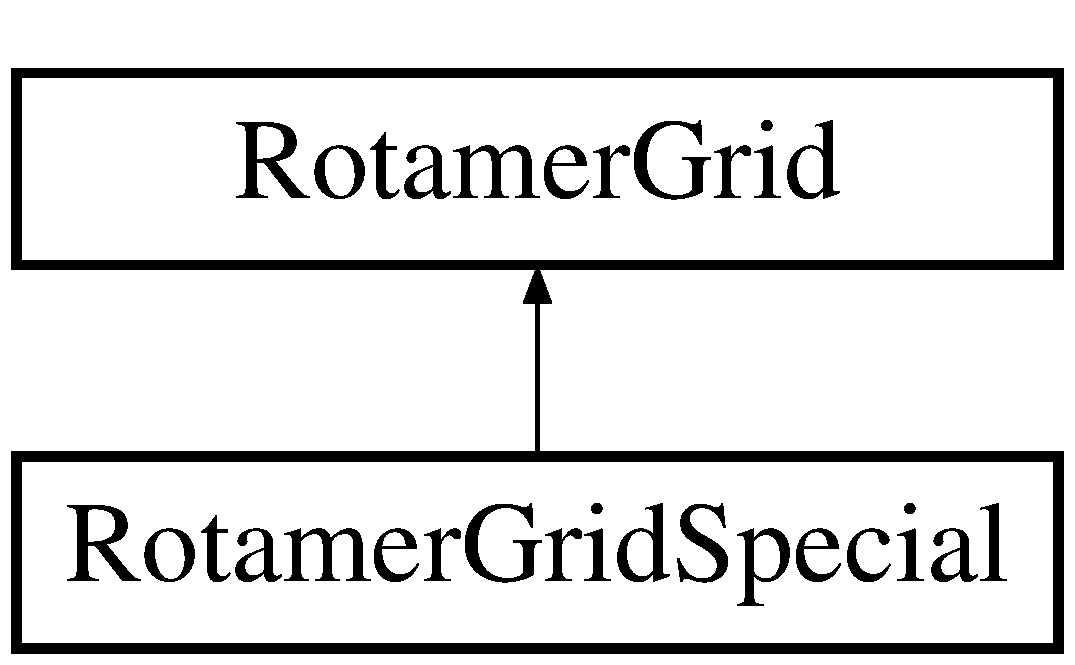
\includegraphics[height=2.000000cm]{classRotamerGridSpecial}
\end{center}
\end{figure}
\subsection*{Public Member Functions}
\begin{DoxyCompactItemize}
\item 
\hypertarget{classRotamerGridSpecial_a072d5082c0eaa6cd68f33e33fbdbf9c2}{bool {\bfseries check} () const }\label{classRotamerGridSpecial_a072d5082c0eaa6cd68f33e33fbdbf9c2}

\end{DoxyCompactItemize}
\subsection*{Public Attributes}
\begin{DoxyCompactItemize}
\item 
\hypertarget{classRotamerGridSpecial_ac53c32c3b34fc7e3976582495e7dea0e}{int {\bfseries degree\-\_\-begin}}\label{classRotamerGridSpecial_ac53c32c3b34fc7e3976582495e7dea0e}

\item 
\hypertarget{classRotamerGridSpecial_aaf8c4aa2c1d5e45210a956cdbb65f089}{int {\bfseries degree\-\_\-end}}\label{classRotamerGridSpecial_aaf8c4aa2c1d5e45210a956cdbb65f089}

\item 
\hypertarget{classRotamerGridSpecial_a996558f134a1a036d40a7496f31b2617}{int {\bfseries step\-Length}}\label{classRotamerGridSpecial_a996558f134a1a036d40a7496f31b2617}

\item 
\hypertarget{classRotamerGridSpecial_aafe50c2b3a85df7bc1debc93d92c503a}{vector$<$ double $>$ {\bfseries dist\-\_\-terminal}}\label{classRotamerGridSpecial_aafe50c2b3a85df7bc1debc93d92c503a}

\item 
\hypertarget{classRotamerGridSpecial_a1898f65ca5d119c65da2a60a39d4fdbf}{vector$<$ vector$<$ double $>$ $>$ {\bfseries acc\-\_\-terminal}}\label{classRotamerGridSpecial_a1898f65ca5d119c65da2a60a39d4fdbf}

\item 
\hypertarget{classRotamerGridSpecial_ab833292e5da159102caef3cbc29aedd2}{vector$<$ vector$<$ double $>$ $>$ {\bfseries chi\-\_\-terminal}}\label{classRotamerGridSpecial_ab833292e5da159102caef3cbc29aedd2}

\end{DoxyCompactItemize}
\subsection*{Friends}
\begin{DoxyCompactItemize}
\item 
\hypertarget{classRotamerGridSpecial_abbb5e1f6ca569c67c8a354f8698eb62e}{class {\bfseries Rotamer}}\label{classRotamerGridSpecial_abbb5e1f6ca569c67c8a354f8698eb62e}

\end{DoxyCompactItemize}


\subsection{Detailed Description}
An auxilliary class for class \hyperlink{classRotamer}{Rotamer}. This class extends \hyperlink{classRotamerGrid}{Rotamer\-Grid} and it adds additional structures for storing non-\/rotameric residues \{A\-S\-N, A\-S\-P, P\-H\-E, T\-R\-P, H\-I\-S, T\-Y\-R, G\-L\-N, G\-L\-U\}. 

The documentation for this class was generated from the following file\-:\begin{DoxyCompactItemize}
\item 
Rotamer.\-h\end{DoxyCompactItemize}

\hypertarget{classSamplePrior}{\section{Sample\-Prior Class Reference}
\label{classSamplePrior}\index{Sample\-Prior@{Sample\-Prior}}
}
Inheritance diagram for Sample\-Prior\-:\begin{figure}[H]
\begin{center}
\leavevmode
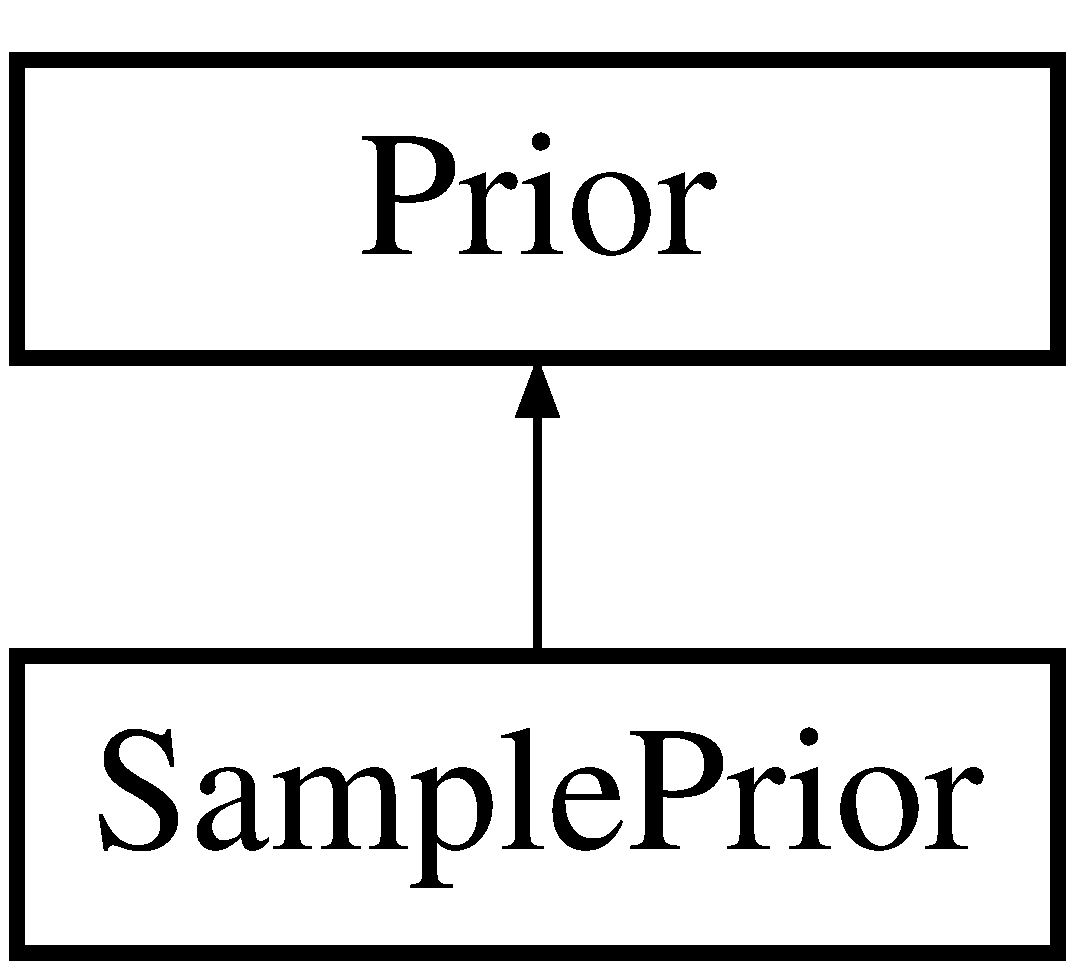
\includegraphics[height=2.000000cm]{classSamplePrior}
\end{center}
\end{figure}
\subsection*{Public Member Functions}
\begin{DoxyCompactItemize}
\item 
double \hyperlink{classSamplePrior_af1209bf9710e4c336084c18b3eba3547}{evaluate} (P\-Chain $\ast$chain)
\begin{DoxyCompactList}\small\item\em Override this function to define custom energy/prior function. \end{DoxyCompactList}\end{DoxyCompactItemize}


\subsection{Member Function Documentation}
\hypertarget{classSamplePrior_af1209bf9710e4c336084c18b3eba3547}{\index{Sample\-Prior@{Sample\-Prior}!evaluate@{evaluate}}
\index{evaluate@{evaluate}!SamplePrior@{Sample\-Prior}}
\subsubsection[{evaluate}]{\setlength{\rightskip}{0pt plus 5cm}double Sample\-Prior\-::evaluate (
\begin{DoxyParamCaption}
\item[{P\-Chain $\ast$}]{protein}
\end{DoxyParamCaption}
)\hspace{0.3cm}{\ttfamily [virtual]}}}\label{classSamplePrior_af1209bf9710e4c336084c18b3eba3547}


Override this function to define custom energy/prior function. 

\begin{DoxyReturn}{Returns}
Probability density in logarithm. 
\end{DoxyReturn}


Reimplemented from \hyperlink{classPrior_a4c130ca9913663eb13d423045640345f}{Prior}.



The documentation for this class was generated from the following file\-:\begin{DoxyCompactItemize}
\item 
main.\-cc\end{DoxyCompactItemize}

\input{classSidechainRotater}
\hypertarget{classSLIKMCSampler}{\section{S\-L\-I\-K\-M\-C\-Sampler Class Reference}
\label{classSLIKMCSampler}\index{S\-L\-I\-K\-M\-C\-Sampler@{S\-L\-I\-K\-M\-C\-Sampler}}
}


Sub-\/\-Loop Inverse Kinematic Markov Chain (S\-L\-I\-K\-M\-C) sampler. Support chain/subchain close-\/loop sampling, free-\/end sampling. Side-\/chain sampling is also supported.  




{\ttfamily \#include $<$S\-L\-I\-K\-M\-C.\-h$>$}

\subsection*{Public Member Functions}
\begin{DoxyCompactItemize}
\item 
\hypertarget{classSLIKMCSampler_af3e1290fab6f427f262aa8eecc07d3b0}{\hyperlink{classSLIKMCSampler_af3e1290fab6f427f262aa8eecc07d3b0}{S\-L\-I\-K\-M\-C\-Sampler} (P\-Protein $\ast$chain)}\label{classSLIKMCSampler_af3e1290fab6f427f262aa8eecc07d3b0}

\begin{DoxyCompactList}\small\item\em Construct a S\-L\-I\-K\-M\-C sampler for specific chain. \end{DoxyCompactList}\item 
\hypertarget{classSLIKMCSampler_a371e96a0e8c02751ac24d00f734ed451}{virtual \hyperlink{classSLIKMCSampler_a371e96a0e8c02751ac24d00f734ed451}{$\sim$\-S\-L\-I\-K\-M\-C\-Sampler} ()}\label{classSLIKMCSampler_a371e96a0e8c02751ac24d00f734ed451}

\begin{DoxyCompactList}\small\item\em Destructor. \end{DoxyCompactList}\item 
void \hyperlink{classSLIKMCSampler_a38e16552bc3531e1385aad7c13aebb63}{sample} (const double time, const int s, const int e)
\begin{DoxyCompactList}\small\item\em Sample conformations of sub-\/loop from residue s to residue e. \end{DoxyCompactList}\item 
void \hyperlink{classSLIKMCSampler_ac093b0714e10dcfe317ba827f0fe13f8}{enable\-Bfactors} (P\-Protein $\ast$chain=N\-U\-L\-L)
\begin{DoxyCompactList}\small\item\em Enable using B-\/factors as priors. \end{DoxyCompactList}\item 
\hypertarget{classSLIKMCSampler_a9d9db8cd58a9e7f56069fd37c8b92841}{void \hyperlink{classSLIKMCSampler_a9d9db8cd58a9e7f56069fd37c8b92841}{disable\-Bfactors} ()}\label{classSLIKMCSampler_a9d9db8cd58a9e7f56069fd37c8b92841}

\begin{DoxyCompactList}\small\item\em Disable using B-\/factors as priors. \end{DoxyCompactList}\item 
\hypertarget{classSLIKMCSampler_a1bd6fa06f57694595e881e3898d5550b}{void \hyperlink{classSLIKMCSampler_a1bd6fa06f57694595e881e3898d5550b}{enable\-Sidechain} ()}\label{classSLIKMCSampler_a1bd6fa06f57694595e881e3898d5550b}

\begin{DoxyCompactList}\small\item\em Enable side-\/chain conformation sampling. \end{DoxyCompactList}\item 
\hypertarget{classSLIKMCSampler_acf98f472f17ea0c02faf11d74ff5db04}{void \hyperlink{classSLIKMCSampler_acf98f472f17ea0c02faf11d74ff5db04}{disable\-Sidechain} ()}\label{classSLIKMCSampler_acf98f472f17ea0c02faf11d74ff5db04}

\begin{DoxyCompactList}\small\item\em Disable side-\/chain in sampling. \end{DoxyCompactList}\item 
\hypertarget{classSLIKMCSampler_aaea4167125ba80b2895a710057c27e4f}{void \hyperlink{classSLIKMCSampler_aaea4167125ba80b2895a710057c27e4f}{enable\-Free\-End} ()}\label{classSLIKMCSampler_aaea4167125ba80b2895a710057c27e4f}

\begin{DoxyCompactList}\small\item\em Enable free-\/end sampling (terminal atoms will stay at fixed positions). \end{DoxyCompactList}\item 
\hypertarget{classSLIKMCSampler_a99f028b7568d863f4f9b25b34633ff01}{void \hyperlink{classSLIKMCSampler_a99f028b7568d863f4f9b25b34633ff01}{disable\-Free\-End} ()}\label{classSLIKMCSampler_a99f028b7568d863f4f9b25b34633ff01}

\begin{DoxyCompactList}\small\item\em Disable free-\/end sampling. \end{DoxyCompactList}\item 
void \hyperlink{classSLIKMCSampler_a1d9ae418449460c7c4f36ac3b3b17662}{enable\-Log} (const int skip=0)
\begin{DoxyCompactList}\small\item\em Enable saving generated conformations. \end{DoxyCompactList}\item 
\hypertarget{classSLIKMCSampler_abf552bb2fcf7df9296d0938f5f455da8}{void \hyperlink{classSLIKMCSampler_abf552bb2fcf7df9296d0938f5f455da8}{disable\-Log} ()}\label{classSLIKMCSampler_abf552bb2fcf7df9296d0938f5f455da8}

\begin{DoxyCompactList}\small\item\em Disable saving generated conformations. \end{DoxyCompactList}\item 
\hypertarget{classSLIKMCSampler_a50b09332cbd488f13bbe26aeac3f0eb0}{void \hyperlink{classSLIKMCSampler_a50b09332cbd488f13bbe26aeac3f0eb0}{enable\-Collision\-Checking} ()}\label{classSLIKMCSampler_a50b09332cbd488f13bbe26aeac3f0eb0}

\begin{DoxyCompactList}\small\item\em Enable steric clash checking for samples. \end{DoxyCompactList}\item 
\hypertarget{classSLIKMCSampler_ac6ccd675c5f5035b41de865219fdee7d}{void \hyperlink{classSLIKMCSampler_ac6ccd675c5f5035b41de865219fdee7d}{disable\-Collision\-Checking} ()}\label{classSLIKMCSampler_ac6ccd675c5f5035b41de865219fdee7d}

\begin{DoxyCompactList}\small\item\em Disable steric clash checking for samples. \end{DoxyCompactList}\item 
\hypertarget{classSLIKMCSampler_a7e71ac082b1d3fcb870cd47745b2e090}{void \hyperlink{classSLIKMCSampler_a7e71ac082b1d3fcb870cd47745b2e090}{enable\-Ramachandran} ()}\label{classSLIKMCSampler_a7e71ac082b1d3fcb870cd47745b2e090}

\begin{DoxyCompactList}\small\item\em Enable using Ramachandran plot as prior. \end{DoxyCompactList}\item 
\hypertarget{classSLIKMCSampler_a13fdd9e0f4aaf23b7ddd3f93dbf8a3eb}{void \hyperlink{classSLIKMCSampler_a13fdd9e0f4aaf23b7ddd3f93dbf8a3eb}{disable\-Ramachandran} ()}\label{classSLIKMCSampler_a13fdd9e0f4aaf23b7ddd3f93dbf8a3eb}

\begin{DoxyCompactList}\small\item\em Disable using Ramachandran plot as prior. \end{DoxyCompactList}\item 
\hypertarget{classSLIKMCSampler_a17c1029a67f4582a31f692652c33cab2}{void \hyperlink{classSLIKMCSampler_a17c1029a67f4582a31f692652c33cab2}{disp\-Settings} ()}\label{classSLIKMCSampler_a17c1029a67f4582a31f692652c33cab2}

\begin{DoxyCompactList}\small\item\em Print current settings for sampling. \end{DoxyCompactList}\item 
\hypertarget{classSLIKMCSampler_a1cf3cb24295225be1bebae24bf3f62c4}{void \hyperlink{classSLIKMCSampler_a1cf3cb24295225be1bebae24bf3f62c4}{enable\-Custom\-Priors} ()}\label{classSLIKMCSampler_a1cf3cb24295225be1bebae24bf3f62c4}

\begin{DoxyCompactList}\small\item\em Enable custom defined priors. \end{DoxyCompactList}\item 
\hypertarget{classSLIKMCSampler_a36f89a31cc6b55113a1adf653fcd273e}{void \hyperlink{classSLIKMCSampler_a36f89a31cc6b55113a1adf653fcd273e}{disable\-Custom\-Priors} ()}\label{classSLIKMCSampler_a36f89a31cc6b55113a1adf653fcd273e}

\begin{DoxyCompactList}\small\item\em Disable custom defined priors. \end{DoxyCompactList}\item 
\hypertarget{classSLIKMCSampler_a3bf93887cc632db16521a4cd21bab7c3}{void \hyperlink{classSLIKMCSampler_a3bf93887cc632db16521a4cd21bab7c3}{add\-Custom\-Prior} (\hyperlink{classPrior}{Prior} \&prior)}\label{classSLIKMCSampler_a3bf93887cc632db16521a4cd21bab7c3}

\begin{DoxyCompactList}\small\item\em Add a custom defined prior. \end{DoxyCompactList}\end{DoxyCompactItemize}
\subsection*{Private Member Functions}
\begin{DoxyCompactItemize}
\item 
bool \hyperlink{classSLIKMCSampler_a4c92bd60cdfd4006b528f652f290fd7a}{M\-H\-Step} (double P, double Q, double P\-\_\-proposal, double Q\-\_\-proposal)
\begin{DoxyCompactList}\small\item\em Metropolis-\/\-Hastings step to decide whether to accept a proposal block. \end{DoxyCompactList}\item 
double \hyperlink{classSLIKMCSampler_a10615e4dc6351319fabbf80ccb329665}{get\-P\-\_\-log} (P\-Protein $\ast$chain)
\begin{DoxyCompactList}\small\item\em Evaluate probability density of one block or sub-\/chain. \end{DoxyCompactList}\item 
double \hyperlink{classSLIKMCSampler_a1ef8cd1fe45f9cd2d188b35133be9e58}{get\-Q\-\_\-log} (P\-Protein $\ast$chain, const int num\-\_\-solutions, int \&status)
\begin{DoxyCompactList}\small\item\em Evaluate proposal density given one block or sub-\/chain. Initial block and proposal block are assumed to be independent. \end{DoxyCompactList}\item 
double \hyperlink{classSLIKMCSampler_a0f35fb022d1a49ced92706301c1c3d80}{get\-Metric\-Tensor\-\_\-log} (P\-Protein $\ast$\hyperlink{classSLIKMCSampler_aa12ccdc8addc18cdb4c48156912811a6}{protein}, int \&status)
\begin{DoxyCompactList}\small\item\em Calculate the metric tensor for one block. \end{DoxyCompactList}\end{DoxyCompactItemize}
\subsection*{Private Attributes}
\begin{DoxyCompactItemize}
\item 
\hypertarget{classSLIKMCSampler_aa12ccdc8addc18cdb4c48156912811a6}{P\-Protein $\ast$ \hyperlink{classSLIKMCSampler_aa12ccdc8addc18cdb4c48156912811a6}{protein}}\label{classSLIKMCSampler_aa12ccdc8addc18cdb4c48156912811a6}

\begin{DoxyCompactList}\small\item\em The protein chain to sample. \end{DoxyCompactList}\item 
\hypertarget{classSLIKMCSampler_a11bbc665e865f9f5c631bce3d823aeb4}{vector$<$ P\-Protein $\ast$ $>$ \hyperlink{classSLIKMCSampler_a11bbc665e865f9f5c631bce3d823aeb4}{subchains}}\label{classSLIKMCSampler_a11bbc665e865f9f5c631bce3d823aeb4}

\begin{DoxyCompactList}\small\item\em Collection of 4-\/residue size blocks. \end{DoxyCompactList}\item 
\hypertarget{classSLIKMCSampler_a9f09703973c780d0c40e9d5e316d746e}{\hyperlink{classBFactor}{B\-Factor} $\ast$ {\bfseries bfactor}}\label{classSLIKMCSampler_a9f09703973c780d0c40e9d5e316d746e}

\item 
\hypertarget{classSLIKMCSampler_af839e7e25e52f980f9aa8b9ed2155f2b}{\hyperlink{classRamachandranPlot}{Ramachandran\-Plot} $\ast$ {\bfseries rplot}}\label{classSLIKMCSampler_af839e7e25e52f980f9aa8b9ed2155f2b}

\item 
\hypertarget{classSLIKMCSampler_a69eaac8ea34ae14a5642f00ab18b5d93}{\hyperlink{classSidechainRotater}{Sidechain\-Rotater} $\ast$ {\bfseries sc\-Rotater}}\label{classSLIKMCSampler_a69eaac8ea34ae14a5642f00ab18b5d93}

\item 
\hypertarget{classSLIKMCSampler_a56dc8f462260c3257badba24c134dcdf}{bool {\bfseries use\-\_\-\-B\-Factor}}\label{classSLIKMCSampler_a56dc8f462260c3257badba24c134dcdf}

\item 
\hypertarget{classSLIKMCSampler_a650506f88623899ce4e76225a4af0ed3}{bool {\bfseries use\-\_\-\-Rotamer}}\label{classSLIKMCSampler_a650506f88623899ce4e76225a4af0ed3}

\item 
\hypertarget{classSLIKMCSampler_ab01d10ae768e4d4fcd2195313fe58a35}{bool {\bfseries free\-End}}\label{classSLIKMCSampler_ab01d10ae768e4d4fcd2195313fe58a35}

\item 
\hypertarget{classSLIKMCSampler_a2e8df530a4b2d3ecf7357417020e969c}{bool {\bfseries use\-\_\-col\-Checking}}\label{classSLIKMCSampler_a2e8df530a4b2d3ecf7357417020e969c}

\item 
\hypertarget{classSLIKMCSampler_a40982641a8d70fb3973c8ec88503ffd7}{bool {\bfseries use\-\_\-\-R\-Plot}}\label{classSLIKMCSampler_a40982641a8d70fb3973c8ec88503ffd7}

\item 
\hypertarget{classSLIKMCSampler_a35c9c56b873e1653d09744c2657067a7}{bool {\bfseries use\-\_\-custom\-Prior}}\label{classSLIKMCSampler_a35c9c56b873e1653d09744c2657067a7}

\item 
\hypertarget{classSLIKMCSampler_aef5a4ce5310270db1948640e246c0db0}{bool {\bfseries init\-\_\-\-Rotamer}}\label{classSLIKMCSampler_aef5a4ce5310270db1948640e246c0db0}

\item 
\hypertarget{classSLIKMCSampler_a1682ebbc84d07ad195853b18a1493826}{bool {\bfseries log\-File}}\label{classSLIKMCSampler_a1682ebbc84d07ad195853b18a1493826}

\item 
\hypertarget{classSLIKMCSampler_adb1ab332267ddb0e87ce22480859c70a}{int {\bfseries skip\-Length}}\label{classSLIKMCSampler_adb1ab332267ddb0e87ce22480859c70a}

\item 
\hypertarget{classSLIKMCSampler_a206a07c1fd82ce6289d8f6b52e1f2c3b}{vector$<$ \hyperlink{classPrior}{Prior} $\ast$ $>$ {\bfseries priors}}\label{classSLIKMCSampler_a206a07c1fd82ce6289d8f6b52e1f2c3b}

\end{DoxyCompactItemize}
\subsection*{Static Private Attributes}
\begin{DoxyCompactItemize}
\item 
\hypertarget{classSLIKMCSampler_a20c7cb30fd8c44b73a1f0b3cdf8a3de0}{static const int \hyperlink{classSLIKMCSampler_a20c7cb30fd8c44b73a1f0b3cdf8a3de0}{M\-A\-X\-\_\-\-I\-K\-\_\-\-S\-A\-M\-P\-L\-E} = 100}\label{classSLIKMCSampler_a20c7cb30fd8c44b73a1f0b3cdf8a3de0}

\begin{DoxyCompactList}\small\item\em Maximum number of dihedral angles we try for the first residue in the subchain in case that I\-K cannot find a solution. \end{DoxyCompactList}\item 
\hypertarget{classSLIKMCSampler_abc1df4b8a822398b575e67dd35912b8d}{static const int \hyperlink{classSLIKMCSampler_abc1df4b8a822398b575e67dd35912b8d}{M\-A\-X\-\_\-\-M\-E\-T\-R\-O\-P\-O\-L\-I\-S\-\_\-\-R\-E\-J\-E\-C\-T} = 1}\label{classSLIKMCSampler_abc1df4b8a822398b575e67dd35912b8d}

\begin{DoxyCompactList}\small\item\em Maximum number of Metropolis Hasting rejects before we giving up. \end{DoxyCompactList}\item 
\hypertarget{classSLIKMCSampler_a2e02967b4a1934c30885da10ce4ca3bf}{static const int \hyperlink{classSLIKMCSampler_a2e02967b4a1934c30885da10ce4ca3bf}{M\-A\-X\-\_\-\-C\-O\-L\-L\-I\-S\-I\-O\-N\-\_\-\-D\-E\-T\-E\-C\-T} = 1}\label{classSLIKMCSampler_a2e02967b4a1934c30885da10ce4ca3bf}

\begin{DoxyCompactList}\small\item\em Maximum number of collision detected before we giving up. \end{DoxyCompactList}\end{DoxyCompactItemize}


\subsection{Detailed Description}
Sub-\/\-Loop Inverse Kinematic Markov Chain (S\-L\-I\-K\-M\-C) sampler. Support chain/subchain close-\/loop sampling, free-\/end sampling. Side-\/chain sampling is also supported. 

\subsection{Member Function Documentation}
\hypertarget{classSLIKMCSampler_ac093b0714e10dcfe317ba827f0fe13f8}{\index{S\-L\-I\-K\-M\-C\-Sampler@{S\-L\-I\-K\-M\-C\-Sampler}!enable\-Bfactors@{enable\-Bfactors}}
\index{enable\-Bfactors@{enable\-Bfactors}!SLIKMCSampler@{S\-L\-I\-K\-M\-C\-Sampler}}
\subsubsection[{enable\-Bfactors}]{\setlength{\rightskip}{0pt plus 5cm}void S\-L\-I\-K\-M\-C\-Sampler\-::enable\-Bfactors (
\begin{DoxyParamCaption}
\item[{P\-Protein $\ast$}]{chain = {\ttfamily NULL}}
\end{DoxyParamCaption}
)}}\label{classSLIKMCSampler_ac093b0714e10dcfe317ba827f0fe13f8}


Enable using B-\/factors as priors. 


\begin{DoxyParams}{Parameters}
{\em chain} & a chain conformation with desired atom positions and B-\/factors \\
\hline
\end{DoxyParams}
\hypertarget{classSLIKMCSampler_a1d9ae418449460c7c4f36ac3b3b17662}{\index{S\-L\-I\-K\-M\-C\-Sampler@{S\-L\-I\-K\-M\-C\-Sampler}!enable\-Log@{enable\-Log}}
\index{enable\-Log@{enable\-Log}!SLIKMCSampler@{S\-L\-I\-K\-M\-C\-Sampler}}
\subsubsection[{enable\-Log}]{\setlength{\rightskip}{0pt plus 5cm}void S\-L\-I\-K\-M\-C\-Sampler\-::enable\-Log (
\begin{DoxyParamCaption}
\item[{const int}]{skip = {\ttfamily 0}}
\end{DoxyParamCaption}
)}}\label{classSLIKMCSampler_a1d9ae418449460c7c4f36ac3b3b17662}


Enable saving generated conformations. 


\begin{DoxyParams}{Parameters}
{\em skip} & number of conformations to skip after last saving conformation. \\
\hline
\end{DoxyParams}
\hypertarget{classSLIKMCSampler_a0f35fb022d1a49ced92706301c1c3d80}{\index{S\-L\-I\-K\-M\-C\-Sampler@{S\-L\-I\-K\-M\-C\-Sampler}!get\-Metric\-Tensor\-\_\-log@{get\-Metric\-Tensor\-\_\-log}}
\index{get\-Metric\-Tensor\-\_\-log@{get\-Metric\-Tensor\-\_\-log}!SLIKMCSampler@{S\-L\-I\-K\-M\-C\-Sampler}}
\subsubsection[{get\-Metric\-Tensor\-\_\-log}]{\setlength{\rightskip}{0pt plus 5cm}double S\-L\-I\-K\-M\-C\-Sampler\-::get\-Metric\-Tensor\-\_\-log (
\begin{DoxyParamCaption}
\item[{P\-Protein $\ast$}]{protein, }
\item[{int \&}]{status}
\end{DoxyParamCaption}
)\hspace{0.3cm}{\ttfamily [private]}}}\label{classSLIKMCSampler_a0f35fb022d1a49ced92706301c1c3d80}


Calculate the metric tensor for one block. 


\begin{DoxyParams}{Parameters}
{\em protein} & a block to be evaluated \\
\hline
{\em status} & an indicator if matrix is not invertible in calculating metric tensor \\
\hline
\end{DoxyParams}
\begin{DoxyReturn}{Returns}

\end{DoxyReturn}
\hypertarget{classSLIKMCSampler_a10615e4dc6351319fabbf80ccb329665}{\index{S\-L\-I\-K\-M\-C\-Sampler@{S\-L\-I\-K\-M\-C\-Sampler}!get\-P\-\_\-log@{get\-P\-\_\-log}}
\index{get\-P\-\_\-log@{get\-P\-\_\-log}!SLIKMCSampler@{S\-L\-I\-K\-M\-C\-Sampler}}
\subsubsection[{get\-P\-\_\-log}]{\setlength{\rightskip}{0pt plus 5cm}double S\-L\-I\-K\-M\-C\-Sampler\-::get\-P\-\_\-log (
\begin{DoxyParamCaption}
\item[{P\-Protein $\ast$}]{chain}
\end{DoxyParamCaption}
)\hspace{0.3cm}{\ttfamily [private]}}}\label{classSLIKMCSampler_a10615e4dc6351319fabbf80ccb329665}


Evaluate probability density of one block or sub-\/chain. 

\begin{DoxyReturn}{Returns}
probability density in logarithm 
\end{DoxyReturn}
\hypertarget{classSLIKMCSampler_a1ef8cd1fe45f9cd2d188b35133be9e58}{\index{S\-L\-I\-K\-M\-C\-Sampler@{S\-L\-I\-K\-M\-C\-Sampler}!get\-Q\-\_\-log@{get\-Q\-\_\-log}}
\index{get\-Q\-\_\-log@{get\-Q\-\_\-log}!SLIKMCSampler@{S\-L\-I\-K\-M\-C\-Sampler}}
\subsubsection[{get\-Q\-\_\-log}]{\setlength{\rightskip}{0pt plus 5cm}double S\-L\-I\-K\-M\-C\-Sampler\-::get\-Q\-\_\-log (
\begin{DoxyParamCaption}
\item[{P\-Protein $\ast$}]{chain, }
\item[{const int}]{num\-\_\-solutions, }
\item[{int \&}]{status}
\end{DoxyParamCaption}
)\hspace{0.3cm}{\ttfamily [private]}}}\label{classSLIKMCSampler_a1ef8cd1fe45f9cd2d188b35133be9e58}


Evaluate proposal density given one block or sub-\/chain. Initial block and proposal block are assumed to be independent. 


\begin{DoxyParams}{Parameters}
{\em num\-\_\-solutions} & number of I\-K solution for the block or sub-\/chain \\
\hline
{\em status} & an indicator if matrix is not invertible in calculating metric tensor \\
\hline
\end{DoxyParams}
\begin{DoxyReturn}{Returns}
proposal density in logarithm 
\end{DoxyReturn}
\hypertarget{classSLIKMCSampler_a4c92bd60cdfd4006b528f652f290fd7a}{\index{S\-L\-I\-K\-M\-C\-Sampler@{S\-L\-I\-K\-M\-C\-Sampler}!M\-H\-Step@{M\-H\-Step}}
\index{M\-H\-Step@{M\-H\-Step}!SLIKMCSampler@{S\-L\-I\-K\-M\-C\-Sampler}}
\subsubsection[{M\-H\-Step}]{\setlength{\rightskip}{0pt plus 5cm}bool S\-L\-I\-K\-M\-C\-Sampler\-::\-M\-H\-Step (
\begin{DoxyParamCaption}
\item[{double}]{P, }
\item[{double}]{Q, }
\item[{double}]{P\-\_\-proposal, }
\item[{double}]{Q\-\_\-proposal}
\end{DoxyParamCaption}
)\hspace{0.3cm}{\ttfamily [private]}}}\label{classSLIKMCSampler_a4c92bd60cdfd4006b528f652f290fd7a}


Metropolis-\/\-Hastings step to decide whether to accept a proposal block. 


\begin{DoxyParams}{Parameters}
{\em P} & Probability density of initial block \\
\hline
{\em Q} & Proposal density of initial block to proposal block \\
\hline
{\em P\-\_\-proposal} & Probability density of proposal block \\
\hline
{\em Q\-\_\-proposal} & Proposal density of proposal block to initial block \\
\hline
\end{DoxyParams}
\begin{DoxyReturn}{Returns}
true\-: accept; false\-: reject 
\end{DoxyReturn}
\hypertarget{classSLIKMCSampler_a38e16552bc3531e1385aad7c13aebb63}{\index{S\-L\-I\-K\-M\-C\-Sampler@{S\-L\-I\-K\-M\-C\-Sampler}!sample@{sample}}
\index{sample@{sample}!SLIKMCSampler@{S\-L\-I\-K\-M\-C\-Sampler}}
\subsubsection[{sample}]{\setlength{\rightskip}{0pt plus 5cm}void S\-L\-I\-K\-M\-C\-Sampler\-::sample (
\begin{DoxyParamCaption}
\item[{const double}]{time, }
\item[{const int}]{s, }
\item[{const int}]{e}
\end{DoxyParamCaption}
)}}\label{classSLIKMCSampler_a38e16552bc3531e1385aad7c13aebb63}


Sample conformations of sub-\/loop from residue s to residue e. 


\begin{DoxyParams}{Parameters}
{\em time} & time duration for sampling \\
\hline
{\em s} & index of starting residue \\
\hline
{\em e} & index of ending residue \\
\hline
\end{DoxyParams}


The documentation for this class was generated from the following files\-:\begin{DoxyCompactItemize}
\item 
S\-L\-I\-K\-M\-C.\-h\item 
S\-L\-I\-K\-M\-C.\-cc\end{DoxyCompactItemize}

\hypertarget{classString}{\section{String Class Reference}
\label{classString}\index{String@{String}}
}
\subsection*{Static Public Member Functions}
\begin{DoxyCompactItemize}
\item 
\hypertarget{classString_a52bb84f85b50b36dc4b46a2c05bab951}{static string {\bfseries to\-Upper} (const string \&)}\label{classString_a52bb84f85b50b36dc4b46a2c05bab951}

\item 
\hypertarget{classString_a8fbbe0bb56277d1c80f0b39fff84223f}{static string {\bfseries to\-Lower} (const string \&)}\label{classString_a8fbbe0bb56277d1c80f0b39fff84223f}

\end{DoxyCompactItemize}


The documentation for this class was generated from the following files\-:\begin{DoxyCompactItemize}
\item 
Utility.\-h\item 
Utility.\-cc\end{DoxyCompactItemize}

\hypertarget{classStringTokenizer}{\section{String\-Tokenizer Class Reference}
\label{classStringTokenizer}\index{String\-Tokenizer@{String\-Tokenizer}}
}


An auxiliary class. The class String\-Tokenzier is a java style utility class for retrieving tokens separated by delims.  




{\ttfamily \#include $<$Utility.\-h$>$}

\subsection*{Public Member Functions}
\begin{DoxyCompactItemize}
\item 
\hyperlink{classStringTokenizer_a04097390a7c9cddce20824648c17bb52}{String\-Tokenizer} (string s, string delims=\char`\"{}\textbackslash{}t\textbackslash{}n \char`\"{})
\begin{DoxyCompactList}\small\item\em Construct a \hyperlink{classStringTokenizer}{String\-Tokenizer} for specific string. \end{DoxyCompactList}\item 
string \hyperlink{classStringTokenizer_a9c95e7412890819dae3e20f23aaa76be}{next\-Token} ()
\begin{DoxyCompactList}\small\item\em Get the next avaiable token. \end{DoxyCompactList}\item 
bool \hyperlink{classStringTokenizer_aae2b0616e31bf6342f3417677f2a2c83}{has\-More\-Tokens} () const 
\begin{DoxyCompactList}\small\item\em Check if there're more tokens left. \end{DoxyCompactList}\item 
void \hyperlink{classStringTokenizer_a8b60b7ec2a45608e2909c872cf4a462a}{get\-All\-Tokens} (vector$<$ string $>$ \&tokens)
\begin{DoxyCompactList}\small\item\em Get all tokens in the string. \end{DoxyCompactList}\end{DoxyCompactItemize}
\subsection*{Private Attributes}
\begin{DoxyCompactItemize}
\item 
\hypertarget{classStringTokenizer_a607a46c28004c9565580b88228c7135c}{string {\bfseries s}}\label{classStringTokenizer_a607a46c28004c9565580b88228c7135c}

\item 
\hypertarget{classStringTokenizer_ac9429222d794407025e69fbbbbe68f19}{vector$<$ char $>$ {\bfseries delims}}\label{classStringTokenizer_ac9429222d794407025e69fbbbbe68f19}

\item 
\hypertarget{classStringTokenizer_a8ac0d6eab57ac99e312c2475ef36dfc6}{int {\bfseries index}}\label{classStringTokenizer_a8ac0d6eab57ac99e312c2475ef36dfc6}

\end{DoxyCompactItemize}


\subsection{Detailed Description}
An auxiliary class. The class String\-Tokenzier is a java style utility class for retrieving tokens separated by delims. 

\subsection{Constructor \& Destructor Documentation}
\hypertarget{classStringTokenizer_a04097390a7c9cddce20824648c17bb52}{\index{String\-Tokenizer@{String\-Tokenizer}!String\-Tokenizer@{String\-Tokenizer}}
\index{String\-Tokenizer@{String\-Tokenizer}!StringTokenizer@{String\-Tokenizer}}
\subsubsection[{String\-Tokenizer}]{\setlength{\rightskip}{0pt plus 5cm}String\-Tokenizer\-::\-String\-Tokenizer (
\begin{DoxyParamCaption}
\item[{string}]{s, }
\item[{string}]{delims = {\ttfamily \char`\"{}\textbackslash{}t\textbackslash{}n~\char`\"{}}}
\end{DoxyParamCaption}
)}}\label{classStringTokenizer_a04097390a7c9cddce20824648c17bb52}


Construct a \hyperlink{classStringTokenizer}{String\-Tokenizer} for specific string. 


\begin{DoxyParams}{Parameters}
{\em s} & string \\
\hline
{\em delims} & characters considered as separators. \\
\hline
\end{DoxyParams}


\subsection{Member Function Documentation}
\hypertarget{classStringTokenizer_a8b60b7ec2a45608e2909c872cf4a462a}{\index{String\-Tokenizer@{String\-Tokenizer}!get\-All\-Tokens@{get\-All\-Tokens}}
\index{get\-All\-Tokens@{get\-All\-Tokens}!StringTokenizer@{String\-Tokenizer}}
\subsubsection[{get\-All\-Tokens}]{\setlength{\rightskip}{0pt plus 5cm}void String\-Tokenizer\-::get\-All\-Tokens (
\begin{DoxyParamCaption}
\item[{vector$<$ string $>$ \&}]{tokens}
\end{DoxyParamCaption}
)}}\label{classStringTokenizer_a8b60b7ec2a45608e2909c872cf4a462a}


Get all tokens in the string. 


\begin{DoxyParams}{Parameters}
{\em tokens} & stores the tokens \\
\hline
\end{DoxyParams}
\hypertarget{classStringTokenizer_aae2b0616e31bf6342f3417677f2a2c83}{\index{String\-Tokenizer@{String\-Tokenizer}!has\-More\-Tokens@{has\-More\-Tokens}}
\index{has\-More\-Tokens@{has\-More\-Tokens}!StringTokenizer@{String\-Tokenizer}}
\subsubsection[{has\-More\-Tokens}]{\setlength{\rightskip}{0pt plus 5cm}bool String\-Tokenizer\-::has\-More\-Tokens (
\begin{DoxyParamCaption}
{}
\end{DoxyParamCaption}
) const}}\label{classStringTokenizer_aae2b0616e31bf6342f3417677f2a2c83}


Check if there're more tokens left. 

\begin{DoxyReturn}{Returns}
true if have more tokens; otherwise false 
\end{DoxyReturn}
\hypertarget{classStringTokenizer_a9c95e7412890819dae3e20f23aaa76be}{\index{String\-Tokenizer@{String\-Tokenizer}!next\-Token@{next\-Token}}
\index{next\-Token@{next\-Token}!StringTokenizer@{String\-Tokenizer}}
\subsubsection[{next\-Token}]{\setlength{\rightskip}{0pt plus 5cm}string String\-Tokenizer\-::next\-Token (
\begin{DoxyParamCaption}
{}
\end{DoxyParamCaption}
)}}\label{classStringTokenizer_a9c95e7412890819dae3e20f23aaa76be}


Get the next avaiable token. 

\begin{DoxyReturn}{Returns}
a token 
\end{DoxyReturn}


The documentation for this class was generated from the following files\-:\begin{DoxyCompactItemize}
\item 
Utility.\-h\item 
Utility.\-cc\end{DoxyCompactItemize}

\hypertarget{classUtility}{\section{Utility Class Reference}
\label{classUtility}\index{Utility@{Utility}}
}


An auxiliary class containing vector and matrix operations.  




{\ttfamily \#include $<$Utility.\-h$>$}

\subsection*{Static Public Member Functions}
\begin{DoxyCompactItemize}
\item 
static void \hyperlink{classUtility_ac9e89b5c673c2627420dcbf32bb1b5e9}{matrix\-\_\-multiply\-\_\-trash} (int m, int n, int p, double $\ast$$\ast$val1, double $\ast$$\ast$val2, double $\ast$$\ast$res, double cov=1)
\item 
\hypertarget{classUtility_a82fddb538f1c8dcb70ef50e98485e198}{static void {\bfseries matrix\-\_\-square\-\_\-transpose\-A} (int m, int n, double $\ast$$\ast$A, double $\ast$$\ast$res)}\label{classUtility_a82fddb538f1c8dcb70ef50e98485e198}

\item 
\hypertarget{classUtility_a149942221766edc56c991eca98b8c1ff}{static double $\ast$$\ast$ {\bfseries new\-\_\-\-Double2\-D} (int m, int n)}\label{classUtility_a149942221766edc56c991eca98b8c1ff}

\item 
\hypertarget{classUtility_a5dd57a755ed7d9644fcf248ca48ba64c}{static void {\bfseries delete\-\_\-\-Double2\-D} (double $\ast$$\ast$values, int m)}\label{classUtility_a5dd57a755ed7d9644fcf248ca48ba64c}

\item 
\hypertarget{classUtility_a8a9ab2f4c25f659b8529d8cd5ae9a833}{static void {\bfseries set\-Zero\-\_\-\-Double2\-D} (int m, int n, double $\ast$$\ast$values)}\label{classUtility_a8a9ab2f4c25f659b8529d8cd5ae9a833}

\item 
\hypertarget{classUtility_a4768fa6de97ffe6f809bc1cd7dd61736}{static double {\bfseries dist} (const vector$<$ double $>$ \&a, const vector$<$ double $>$ \&b, const int minsize)}\label{classUtility_a4768fa6de97ffe6f809bc1cd7dd61736}

\end{DoxyCompactItemize}


\subsection{Detailed Description}
An auxiliary class containing vector and matrix operations. 

\subsection{Member Function Documentation}
\hypertarget{classUtility_ac9e89b5c673c2627420dcbf32bb1b5e9}{\index{Utility@{Utility}!matrix\-\_\-multiply\-\_\-trash@{matrix\-\_\-multiply\-\_\-trash}}
\index{matrix\-\_\-multiply\-\_\-trash@{matrix\-\_\-multiply\-\_\-trash}!Utility@{Utility}}
\subsubsection[{matrix\-\_\-multiply\-\_\-trash}]{\setlength{\rightskip}{0pt plus 5cm}void Utility\-::matrix\-\_\-multiply\-\_\-trash (
\begin{DoxyParamCaption}
\item[{int}]{m, }
\item[{int}]{n, }
\item[{int}]{p, }
\item[{double $\ast$$\ast$}]{val1, }
\item[{double $\ast$$\ast$}]{val2, }
\item[{double $\ast$$\ast$}]{res, }
\item[{double}]{cov = {\ttfamily 1}}
\end{DoxyParamCaption}
)\hspace{0.3cm}{\ttfamily [static]}}}\label{classUtility_ac9e89b5c673c2627420dcbf32bb1b5e9}

\begin{DoxyParams}{Parameters}
{\em m} & \\
\hline
{\em n} & \\
\hline
{\em p} & \\
\hline
{\em val1} & \\
\hline
{\em val2} & \\
\hline
{\em res} & \\
\hline
{\em cov} & \\
\hline
\end{DoxyParams}


The documentation for this class was generated from the following files\-:\begin{DoxyCompactItemize}
\item 
Utility.\-h\item 
Utility.\-cc\end{DoxyCompactItemize}

\addcontentsline{toc}{part}{Index}
\printindex
\end{document}
